\documentclass[11pt,aspectratio=169]{beamer}

%% ---- Theme ----
\usetheme{metropolis}
\usepackage[utf8]{inputenc}
\usepackage[T1]{fontenc}
\usepackage{graphicx}
\usepackage{booktabs}
\usepackage{amsmath}
\usepackage{appendixnumberbeamer}

%% ---- Colors ----
\definecolor{msugreen}{HTML}{18453B}
\definecolor{msugray}{HTML}{97A2A2}
\setbeamercolor{frametitle}{bg=msugreen}
\setbeamercolor{progress bar}{fg=msugreen}
\setbeamercolor{alerted text}{fg=msugreen}

%% ---- Metadata ----
\title{County Vulnerability to SNAP Losses\\Under Expanded ABAWD Work Requirements}
\subtitle{Evidence from Michigan's Staggered Reinstatement}
\author{Jiaming Zhang}
\institute{Department of Agricultural, Food, and Resource Economics\\Michigan State University}
\date{\today}

\begin{document}

% ====================================================================
% TITLE
% ====================================================================
\begin{frame}[plain]
\titlepage
\end{frame}

% ====================================================================
% 1. MOTIVATION & RESEARCH QUESTION  (~1 min)
% ====================================================================
\begin{frame}{Motivation}

\textbf{Policy context}
\begin{itemize}
  \item SNAP ABAWD time limits: 3 months of benefits per 36 months unless working $\geq$80 hrs/month
  \item States received broad waivers after 2008; waivers expired as labor markets recovered
  \item \alert{2026 One Big Beautiful Bill Act (OBBBA)}: work requirements extend to ages \textbf{55--64}
\end{itemize}

\vspace{0.8em}
\textbf{Research question}
\begin{quote}
Which Michigan counties face the greatest risk of SNAP participation losses under expanded work requirements, and what county characteristics predict larger impacts?
\end{quote}

\end{frame}

% ====================================================================
% 2. INSTITUTIONAL SETTING  (~1.5 min)
% ====================================================================
\begin{frame}{Michigan's Staggered Reinstatement}

\begin{columns}[T]
\begin{column}{0.55\textwidth}
\textbf{Four treatment cohorts:}
\begin{enumerate}
  \item \textbf{Jan 2017} --- 4 counties (Kent, Oakland, Ottawa, Washtenaw)
  \item \textbf{Jan 2018} --- 10 counties (suburban/mid-metro)
  \item \textbf{Jul 2018} --- 68 counties (rural, gradual phase-in)
  \item \textbf{Oct 2018} --- 1 county (Wayne/Detroit)
\end{enumerate}

\vspace{0.5em}
$\Rightarrow$ \textbf{All 83 counties} eventually treated\\
$\Rightarrow$ Identification: \emph{not-yet-treated} as controls
\end{column}

\begin{column}{0.42\textwidth}
\centering
\small
\begin{tabular}{lcc}
\toprule
Cohort & Unemp. & Bach. \\
\midrule
Jan 17 & 3.9\% & 40.6\% \\
Jan 18 & 4.4\% & 27.5\% \\
Jul 18 & 6.7\% & 18.2\% \\
Oct 18 & 6.8\% & 22.1\% \\
\bottomrule
\end{tabular}

\vspace{0.5em}
{\footnotesize \textit{Key:} Treatment timing $\sim$ labor market strength $\Rightarrow$ \alert{confounding risk}}
\end{column}
\end{columns}

\end{frame}

% ====================================================================
% 3. DATA  (~1 min)
% ====================================================================
\begin{frame}{Data}

\begin{itemize}
  \item \textbf{Michigan FAP} county-month panel: Jan 2014 -- Dec 2019 (83 counties $\times$ 72 months)
  \item \textbf{Outcome}: $\log(\text{SNAP recipients per 1,000 adults 18--49})$
    \begin{itemize}
      \item Min $\approx 52$/1k (no zeros $\Rightarrow$ log well-defined)
      \item Mean $= 225$/1k; SD $= 94$
    \end{itemize}
  \item \textbf{County characteristics}: BLS unemployment, ACS poverty \& education, CDC SVI, USDA RUCC
  \item \textbf{Estimation sample}: 5,229 county-month obs after trimming anticipation window
\end{itemize}

\end{frame}

% ====================================================================
% 4. EMPIRICAL STRATEGY  (~1.5 min)
% ====================================================================
\begin{frame}{Empirical Strategy}

\textbf{Callaway \& Sant'Anna (2021)} staggered DiD:
\[
ATT(g,t) = \mathbb{E}\bigl[Y_t(g) - Y_t(0) \;\big|\; G = g\bigr]
\]

\begin{itemize}
  \item Control group: \emph{not-yet-treated} counties
  \item Doubly-robust (DR) with unemployment rate as covariate
  \item Anticipation $\delta = 2$ months (waiver removal announced $\sim$4 months early)
  \item Event study: $e \in [-6, +6]$ months
  \item Clustering: county level
\end{itemize}

\vspace{0.5em}
\textbf{Placebo}: DDD comparing adult recipients (affected) vs.\ child recipients (unaffected)

\end{frame}

% ====================================================================
% 5. MAIN RESULTS: EVENT STUDY  (~1.5 min)
% ====================================================================
\begin{frame}{Main Result: Event Study}

\begin{columns}[T]
\begin{column}{0.62\textwidth}
  \centering
  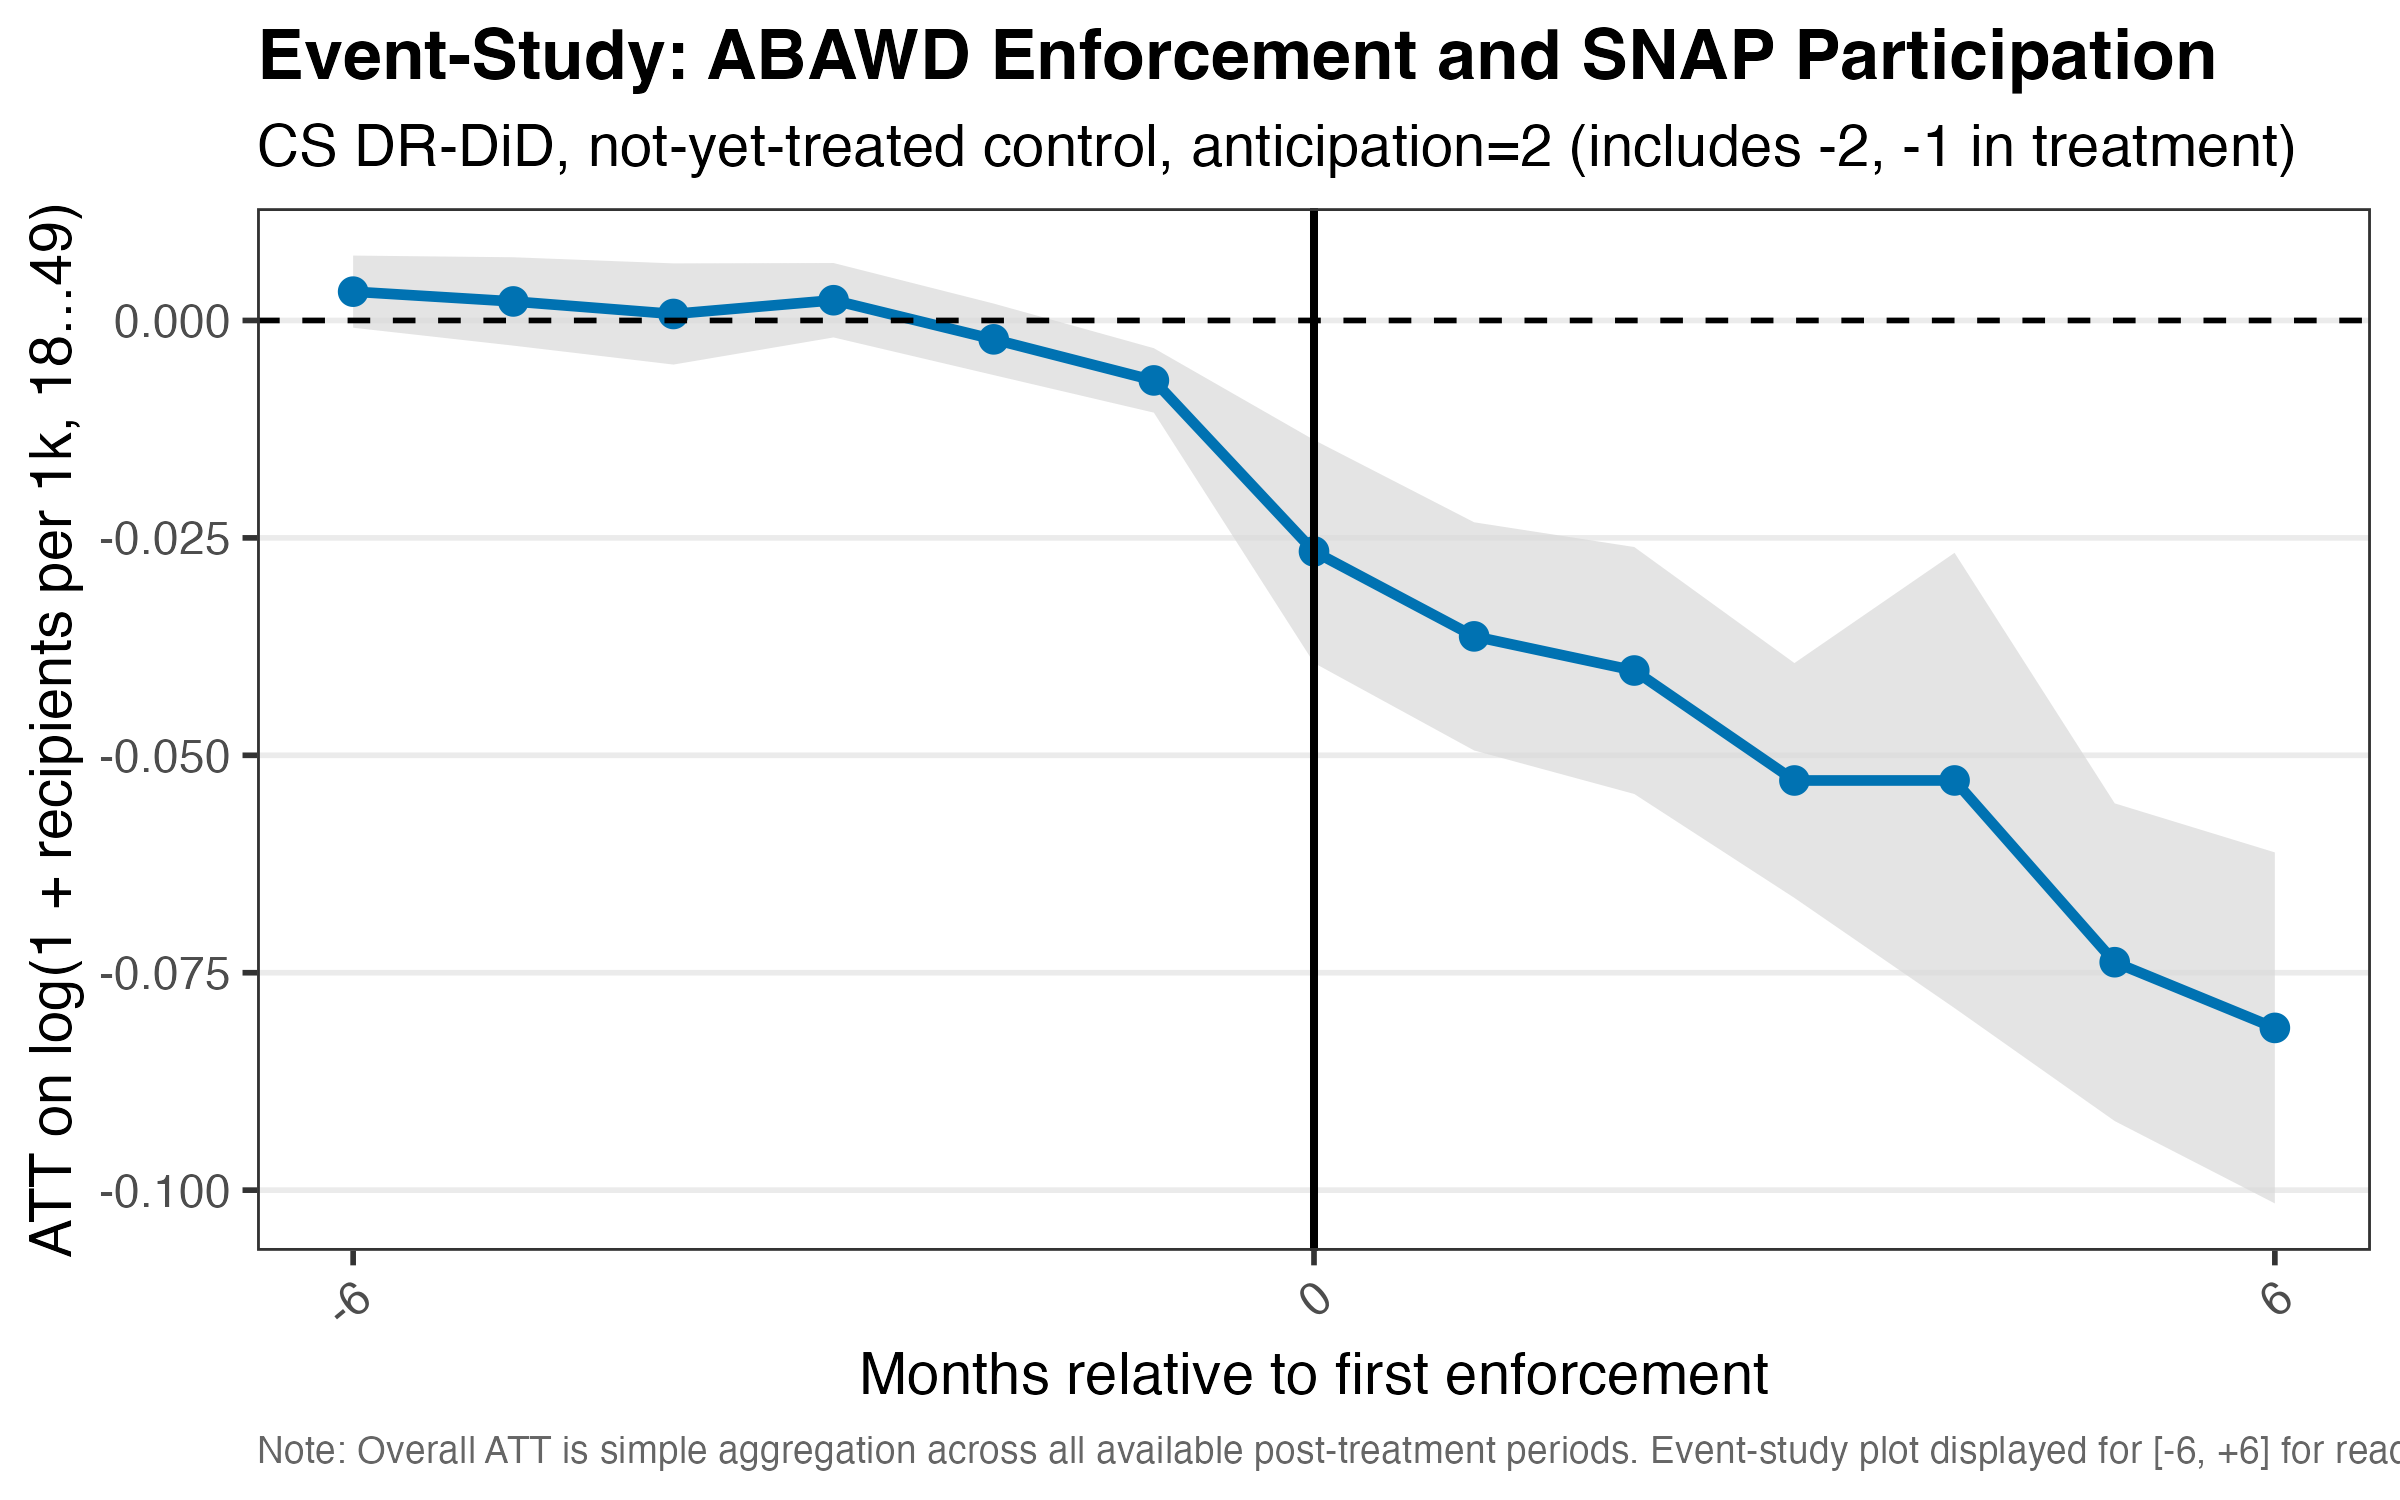
\includegraphics[width=\textwidth]{../outputs/figures/abawd_es_main}
\end{column}
\begin{column}{0.35\textwidth}
  \textbf{Key findings:}
  \begin{itemize}
    \item Pre-trends flat ($e \leq -3$)
    \item Overall ATT $= -0.060$ \\(SE $= 0.010$, $p < 0.01$)
    \item $\approx$ \textbf{5.8\% reduction} in SNAP participation
    \item Effects accumulate over 6 months (recertification phase-in)
  \end{itemize}
\end{column}
\end{columns}

\end{frame}

% ====================================================================
% 6. DDD PLACEBO  (~0.5 min)
% ====================================================================
\begin{frame}{DDD Placebo: Adult vs.\ Child Recipients}

\begin{columns}[T]
\begin{column}{0.62\textwidth}
  \centering
  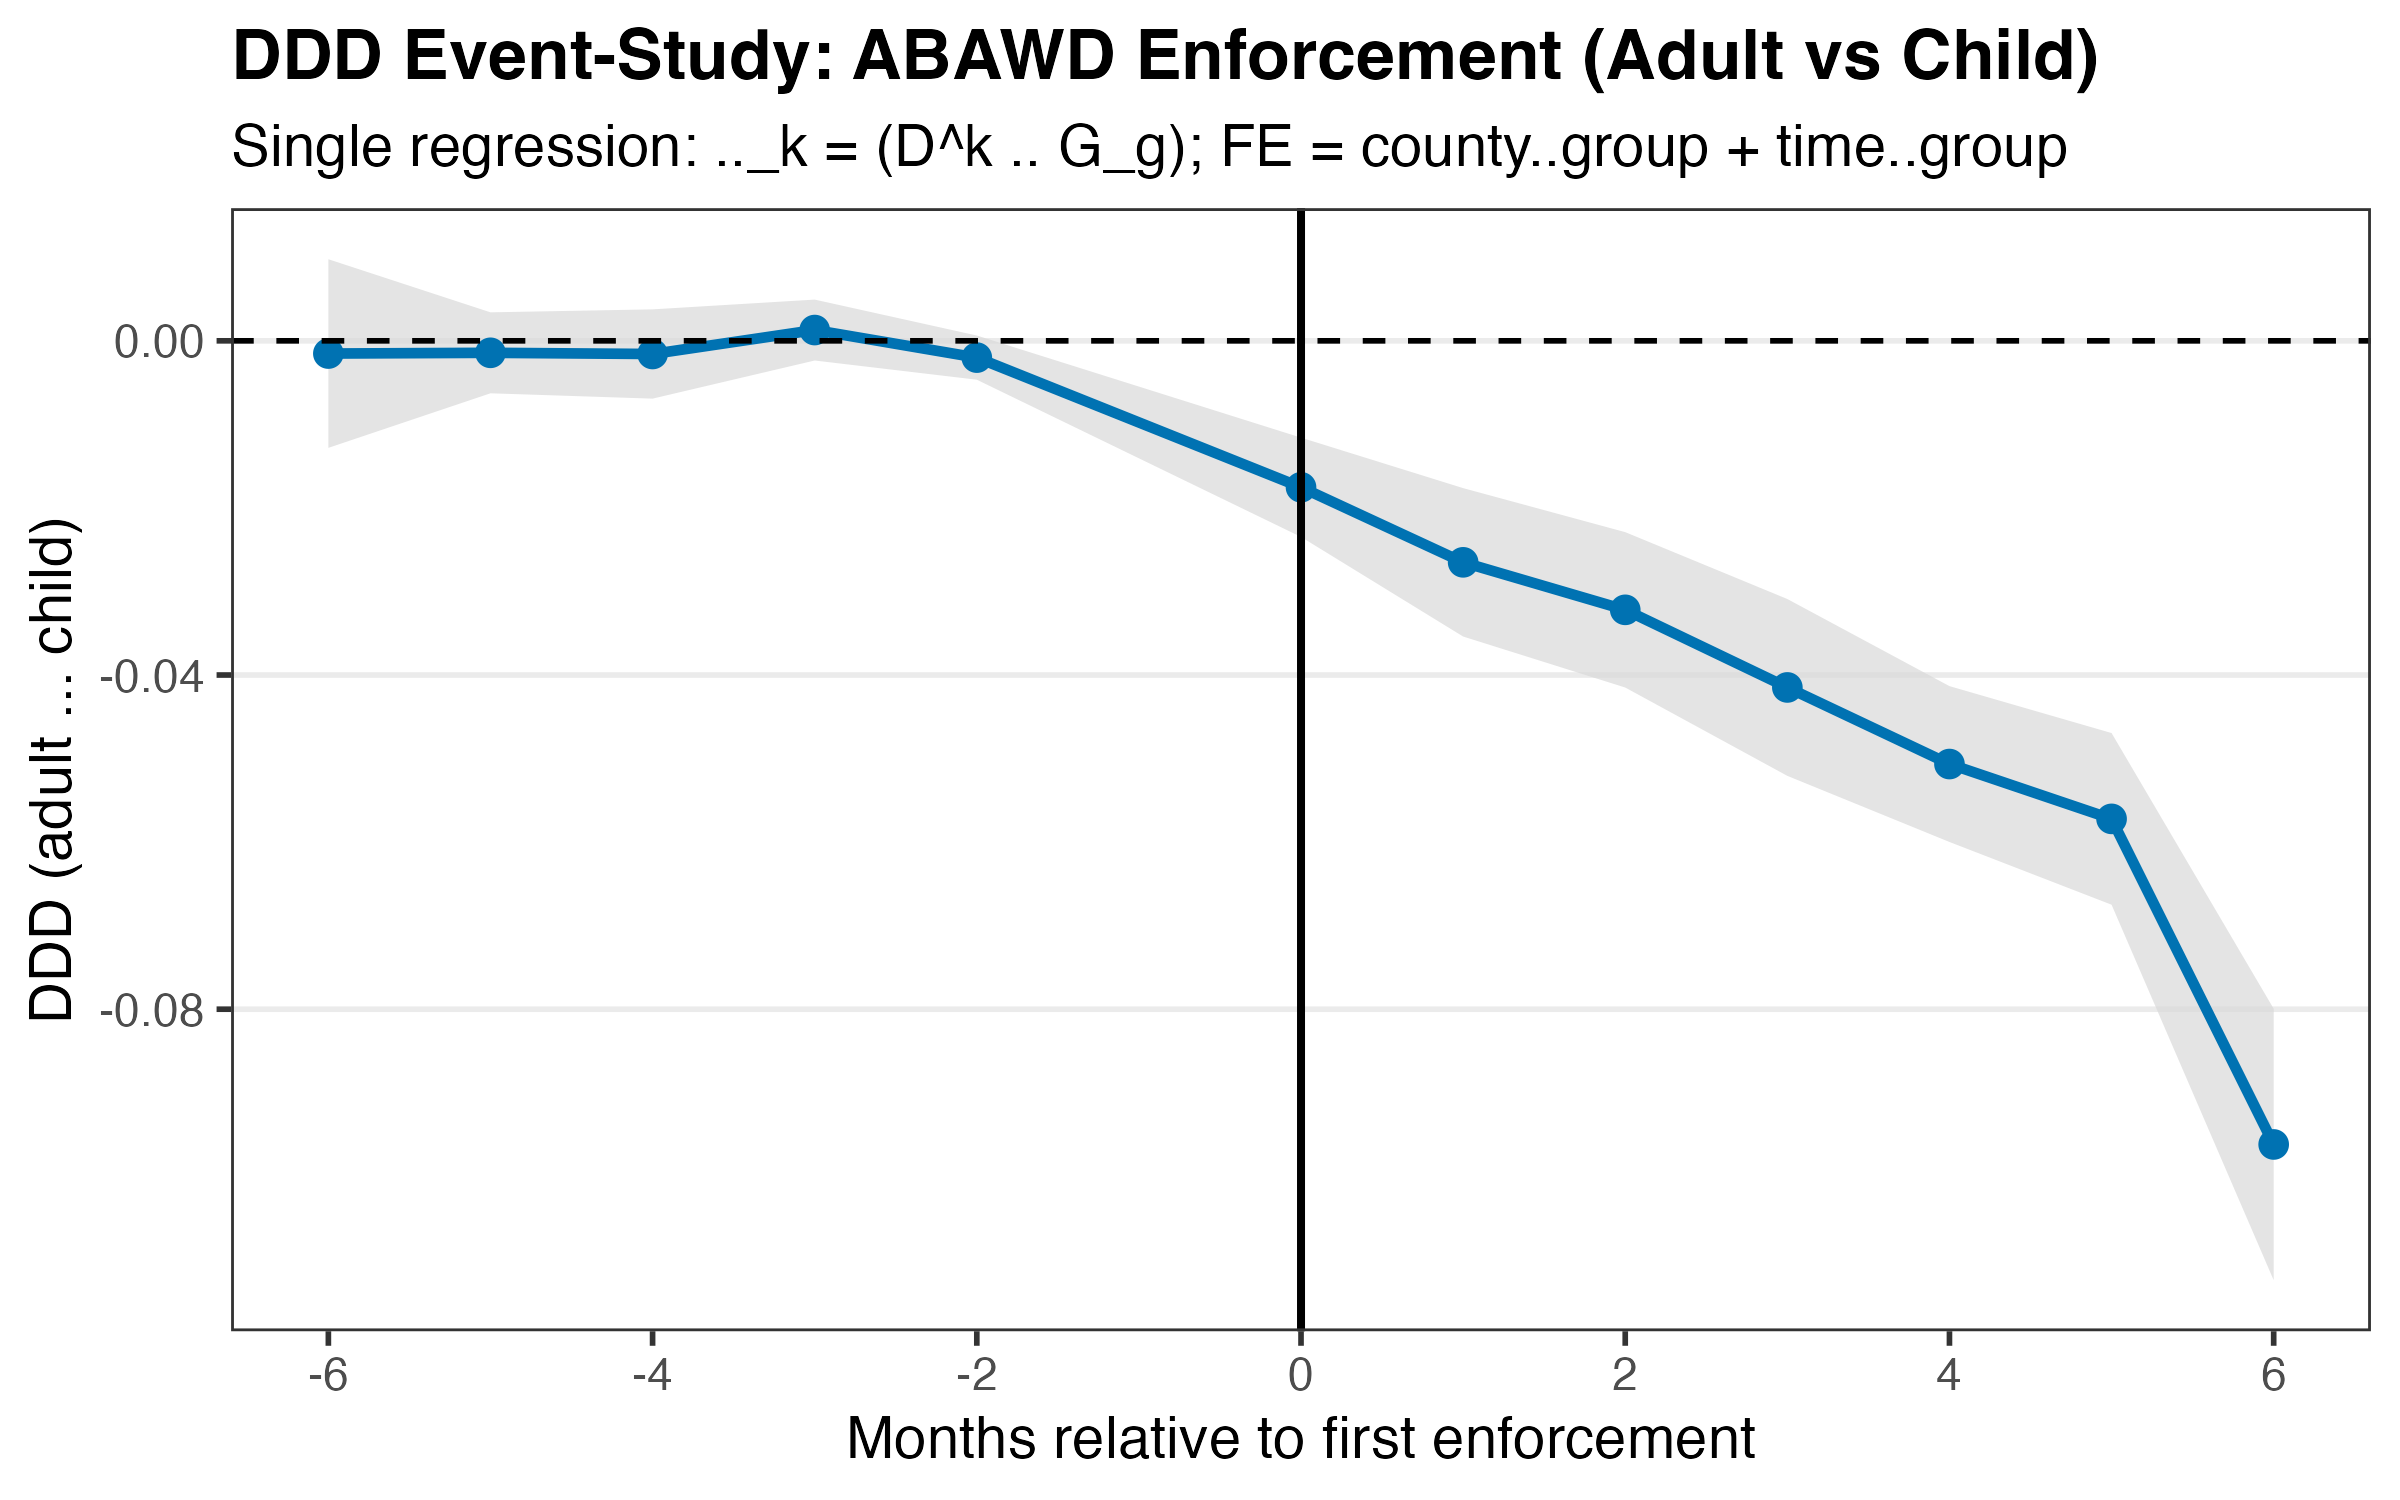
\includegraphics[width=\textwidth]{../outputs/figures/abawd_es_ddd_adult_child}
\end{column}
\begin{column}{0.35\textwidth}
  \begin{itemize}
    \item Adult recipients (subject to ABAWD): \alert{significant decline}
    \item Child recipients (not subject): \textbf{no effect}
    \item Rules out county-level confounders affecting both groups
  \end{itemize}
\end{column}
\end{columns}

\end{frame}

% ====================================================================
% 7. HETEROGENEITY: CONFOUNDING DIAGNOSTIC  (~2 min)
% ====================================================================
\begin{frame}{Heterogeneity: Treatment-Timing Confounding}

\small
\begin{columns}[T]
\begin{column}{0.48\textwidth}
  \centering
  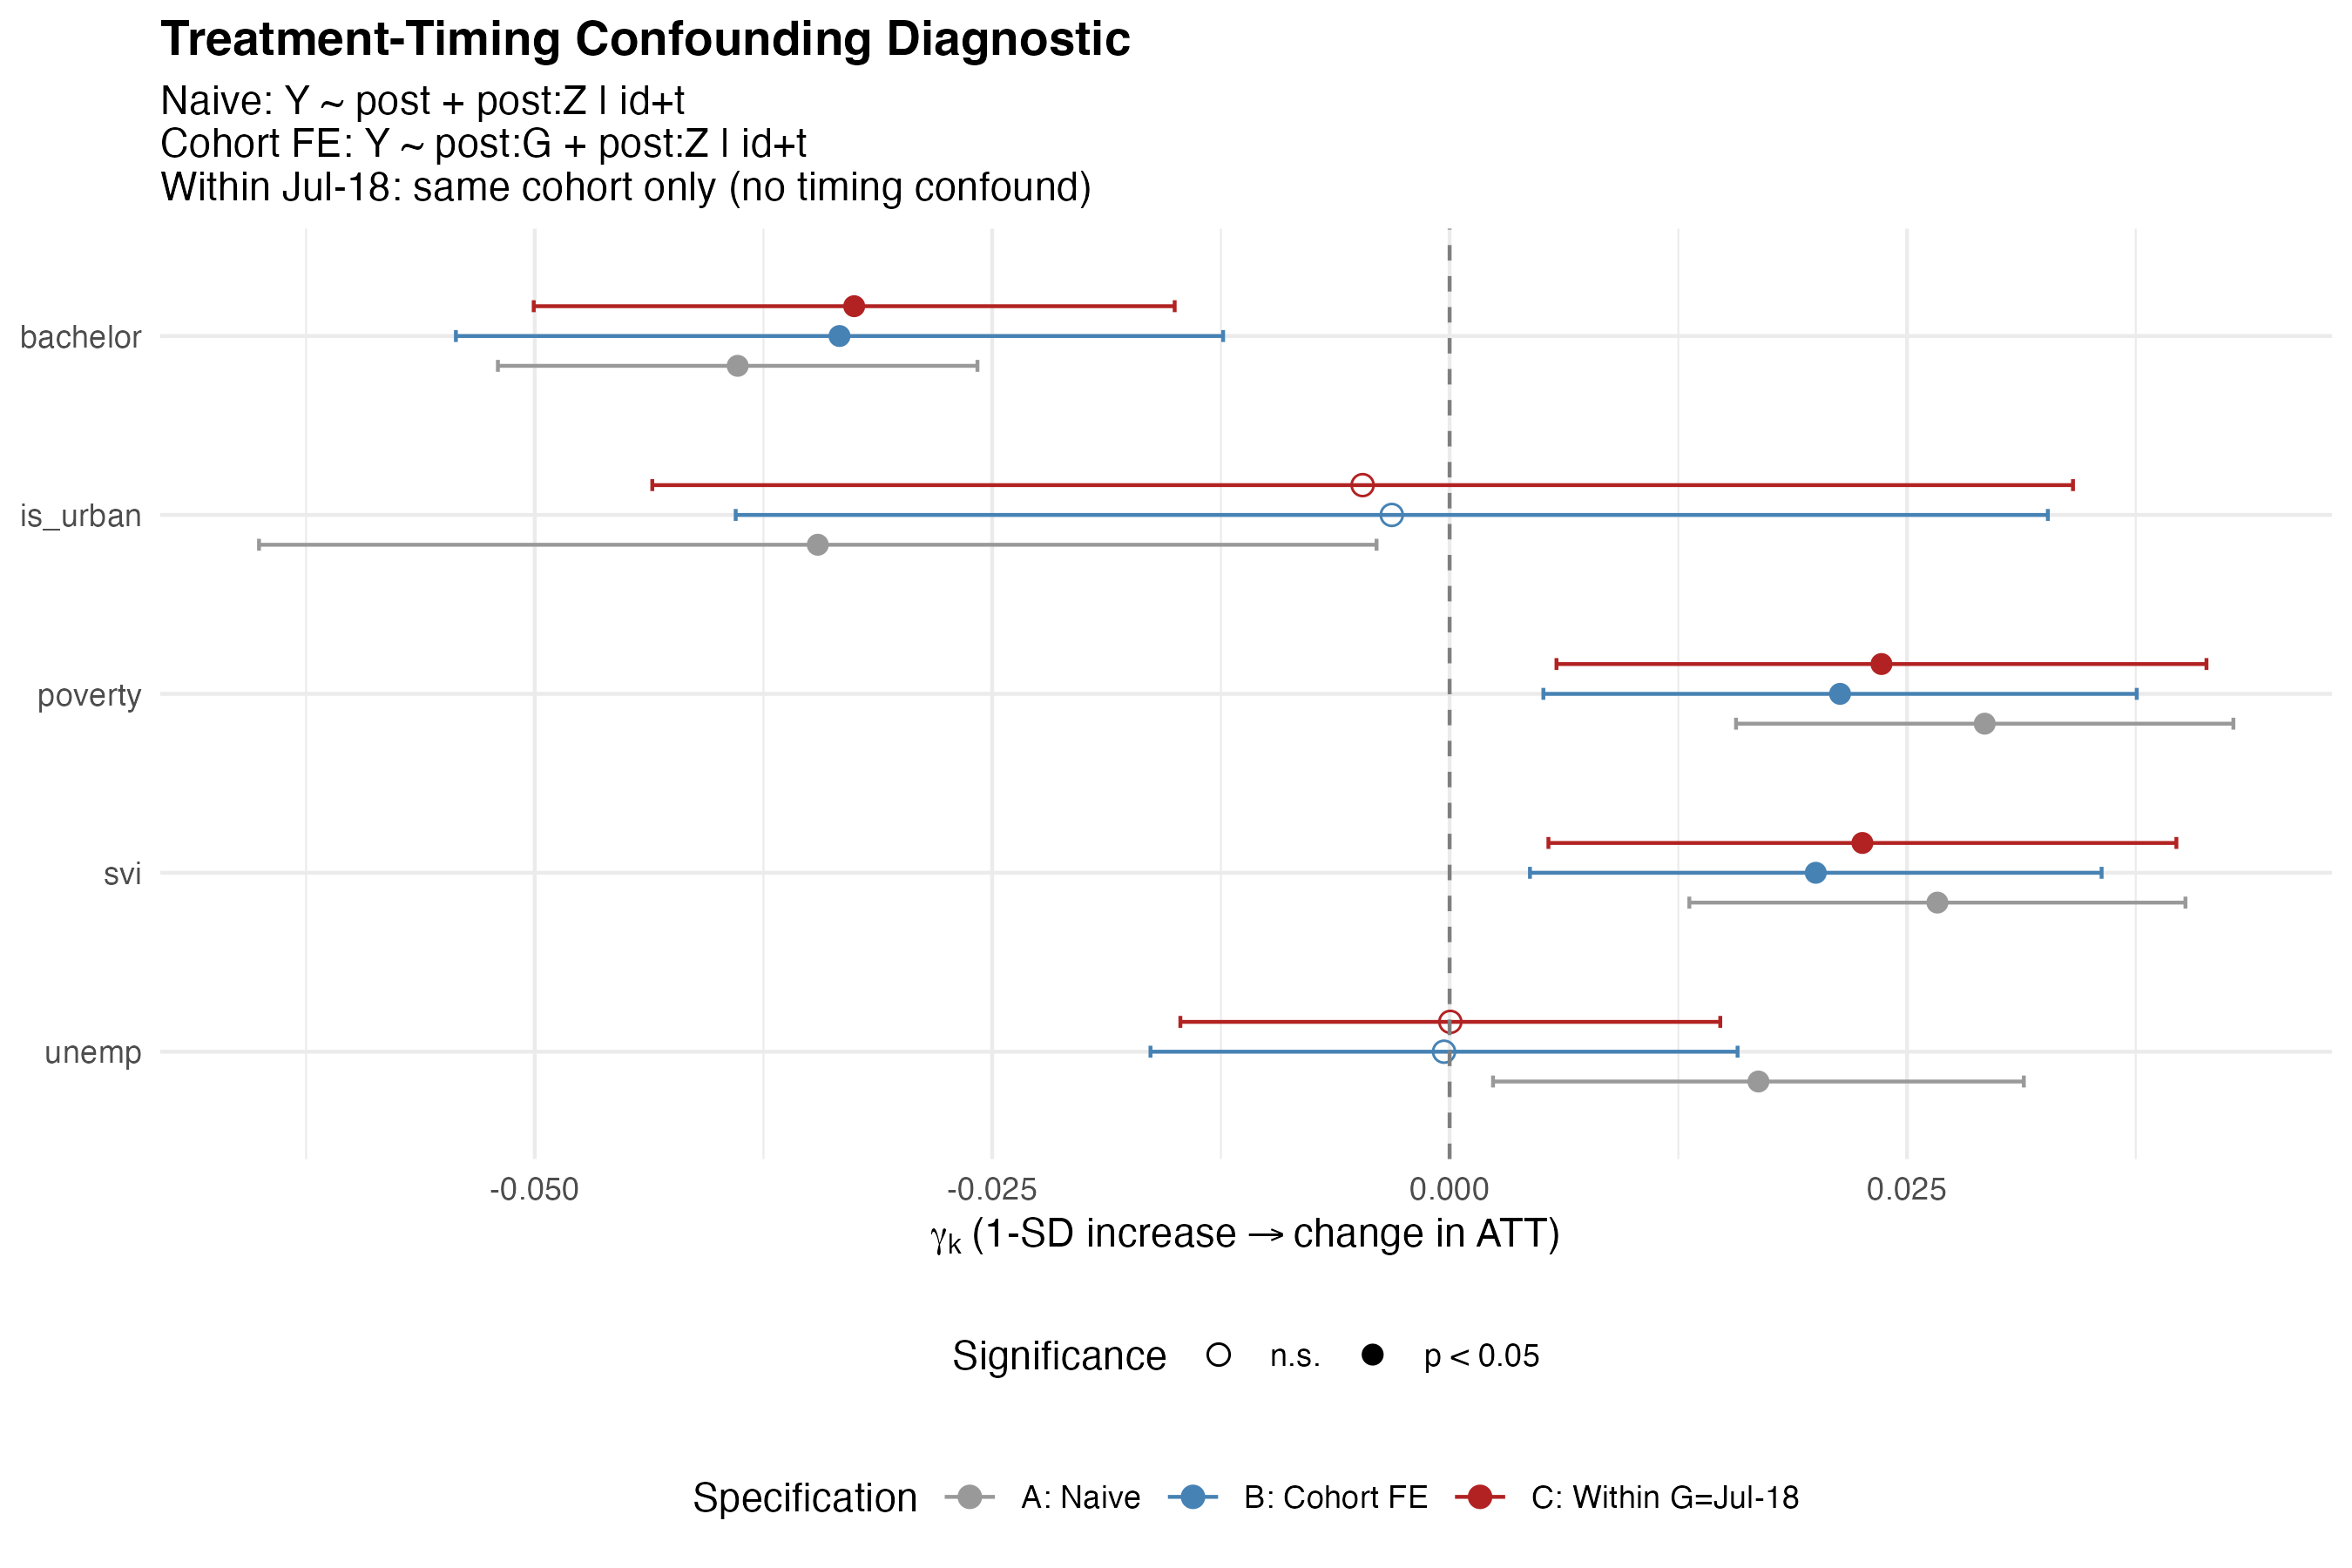
\includegraphics[width=\textwidth]{../outputs/figures/abawd_heterogeneity_interactions}
\end{column}
\begin{column}{0.50\textwidth}
\textbf{Diagnostic:} A.~Naive $\to$ B.~Cohort FE $\to$ C.~Within Jul-18

\vspace{0.4em}
\textbf{Spurious} (vanish in B\,\&\,C):
\begin{itemize}\setlength\itemsep{0em}
  \item Unemployment: $+0.016^{**} \to 0.000$
  \item Urbanicity: $-0.034^{**} \to -0.003$
\end{itemize}

\vspace{0.2em}
\textbf{Genuine} (survive all specs):
\begin{itemize}\setlength\itemsep{0em}
  \item Bachelor's share: $-0.033^{***}$
  \item Poverty rate: $+0.021^{**}$
  \item SVI: $+0.020^{**}$
\end{itemize}

\vspace{0.2em}
{\footnotesize LASSO: selects only bachelor's \& poverty}
\end{column}
\end{columns}

\end{frame}

% ====================================================================
% 8. PROJECTION METHOD  (~1 min)
% ====================================================================
\begin{frame}{Projection: 2026 OBBBA Expansion to Ages 55--64}
\small

\textbf{County-specific predicted ATT} \quad $\widehat{ATT}_c = \overline{ATT} + \hat{\delta}_1 \tilde{Z}^{\text{bach}}_c + \hat{\delta}_2 \tilde{Z}^{\text{pov}}_c$

\textbf{Projected loss} \quad $\widehat{\Delta Y}_c = \widehat{ATT}_c \times S_c^{55\text{-}64} \times \bar{Y}_{c,\text{pre}}$ \hfill {\footnotesize Uncertainty: bootstrap $B = 2{,}000$}

\vspace{0.5em}
\begin{columns}[T]
\begin{column}{0.48\textwidth}
\textbf{Three scenarios:}
\begin{itemize}\setlength\itemsep{0.1em}
  \item Baseline (current unemployment)
  \item Recession (+3 pp unemployment)
  \item Tight labor ($-$2 pp unemployment)
\end{itemize}
\end{column}
\begin{column}{0.48\textwidth}
\textbf{Three channels:}
\begin{itemize}\setlength\itemsep{0.1em}
  \item Compliance: harder to meet 80-hr req
  \item Enrollment: more people on SNAP
  \item Waiver: $>$10\% unemp $\Rightarrow$ exemption
\end{itemize}
\end{column}
\end{columns}

\end{frame}

% ====================================================================
% 9. PROJECTION RESULTS  (~1.5 min)
% ====================================================================
\begin{frame}{Projection Results}

\begin{columns}[T]
\begin{column}{0.48\textwidth}
\centering
\small
\begin{tabular}{lc}
\toprule
Scenario & Total loss \\
\midrule
Baseline              & $-9{,}918$ \\
& {\scriptsize [7,200 -- 12,600]} \\
Recession (+3 pp)     & $-13{,}440$ \\
Tight labor ($-$2 pp) & $-7{,}805$ \\
\bottomrule
\end{tabular}

\vspace{0.8em}
\begin{itemize}
  \item $\sim$\textbf{10,000} individuals projected to lose benefits
  \item Recession amplifies by 36\%
  \item Recovery attenuates by 21\%
\end{itemize}
\end{column}
\begin{column}{0.50\textwidth}
  \centering
  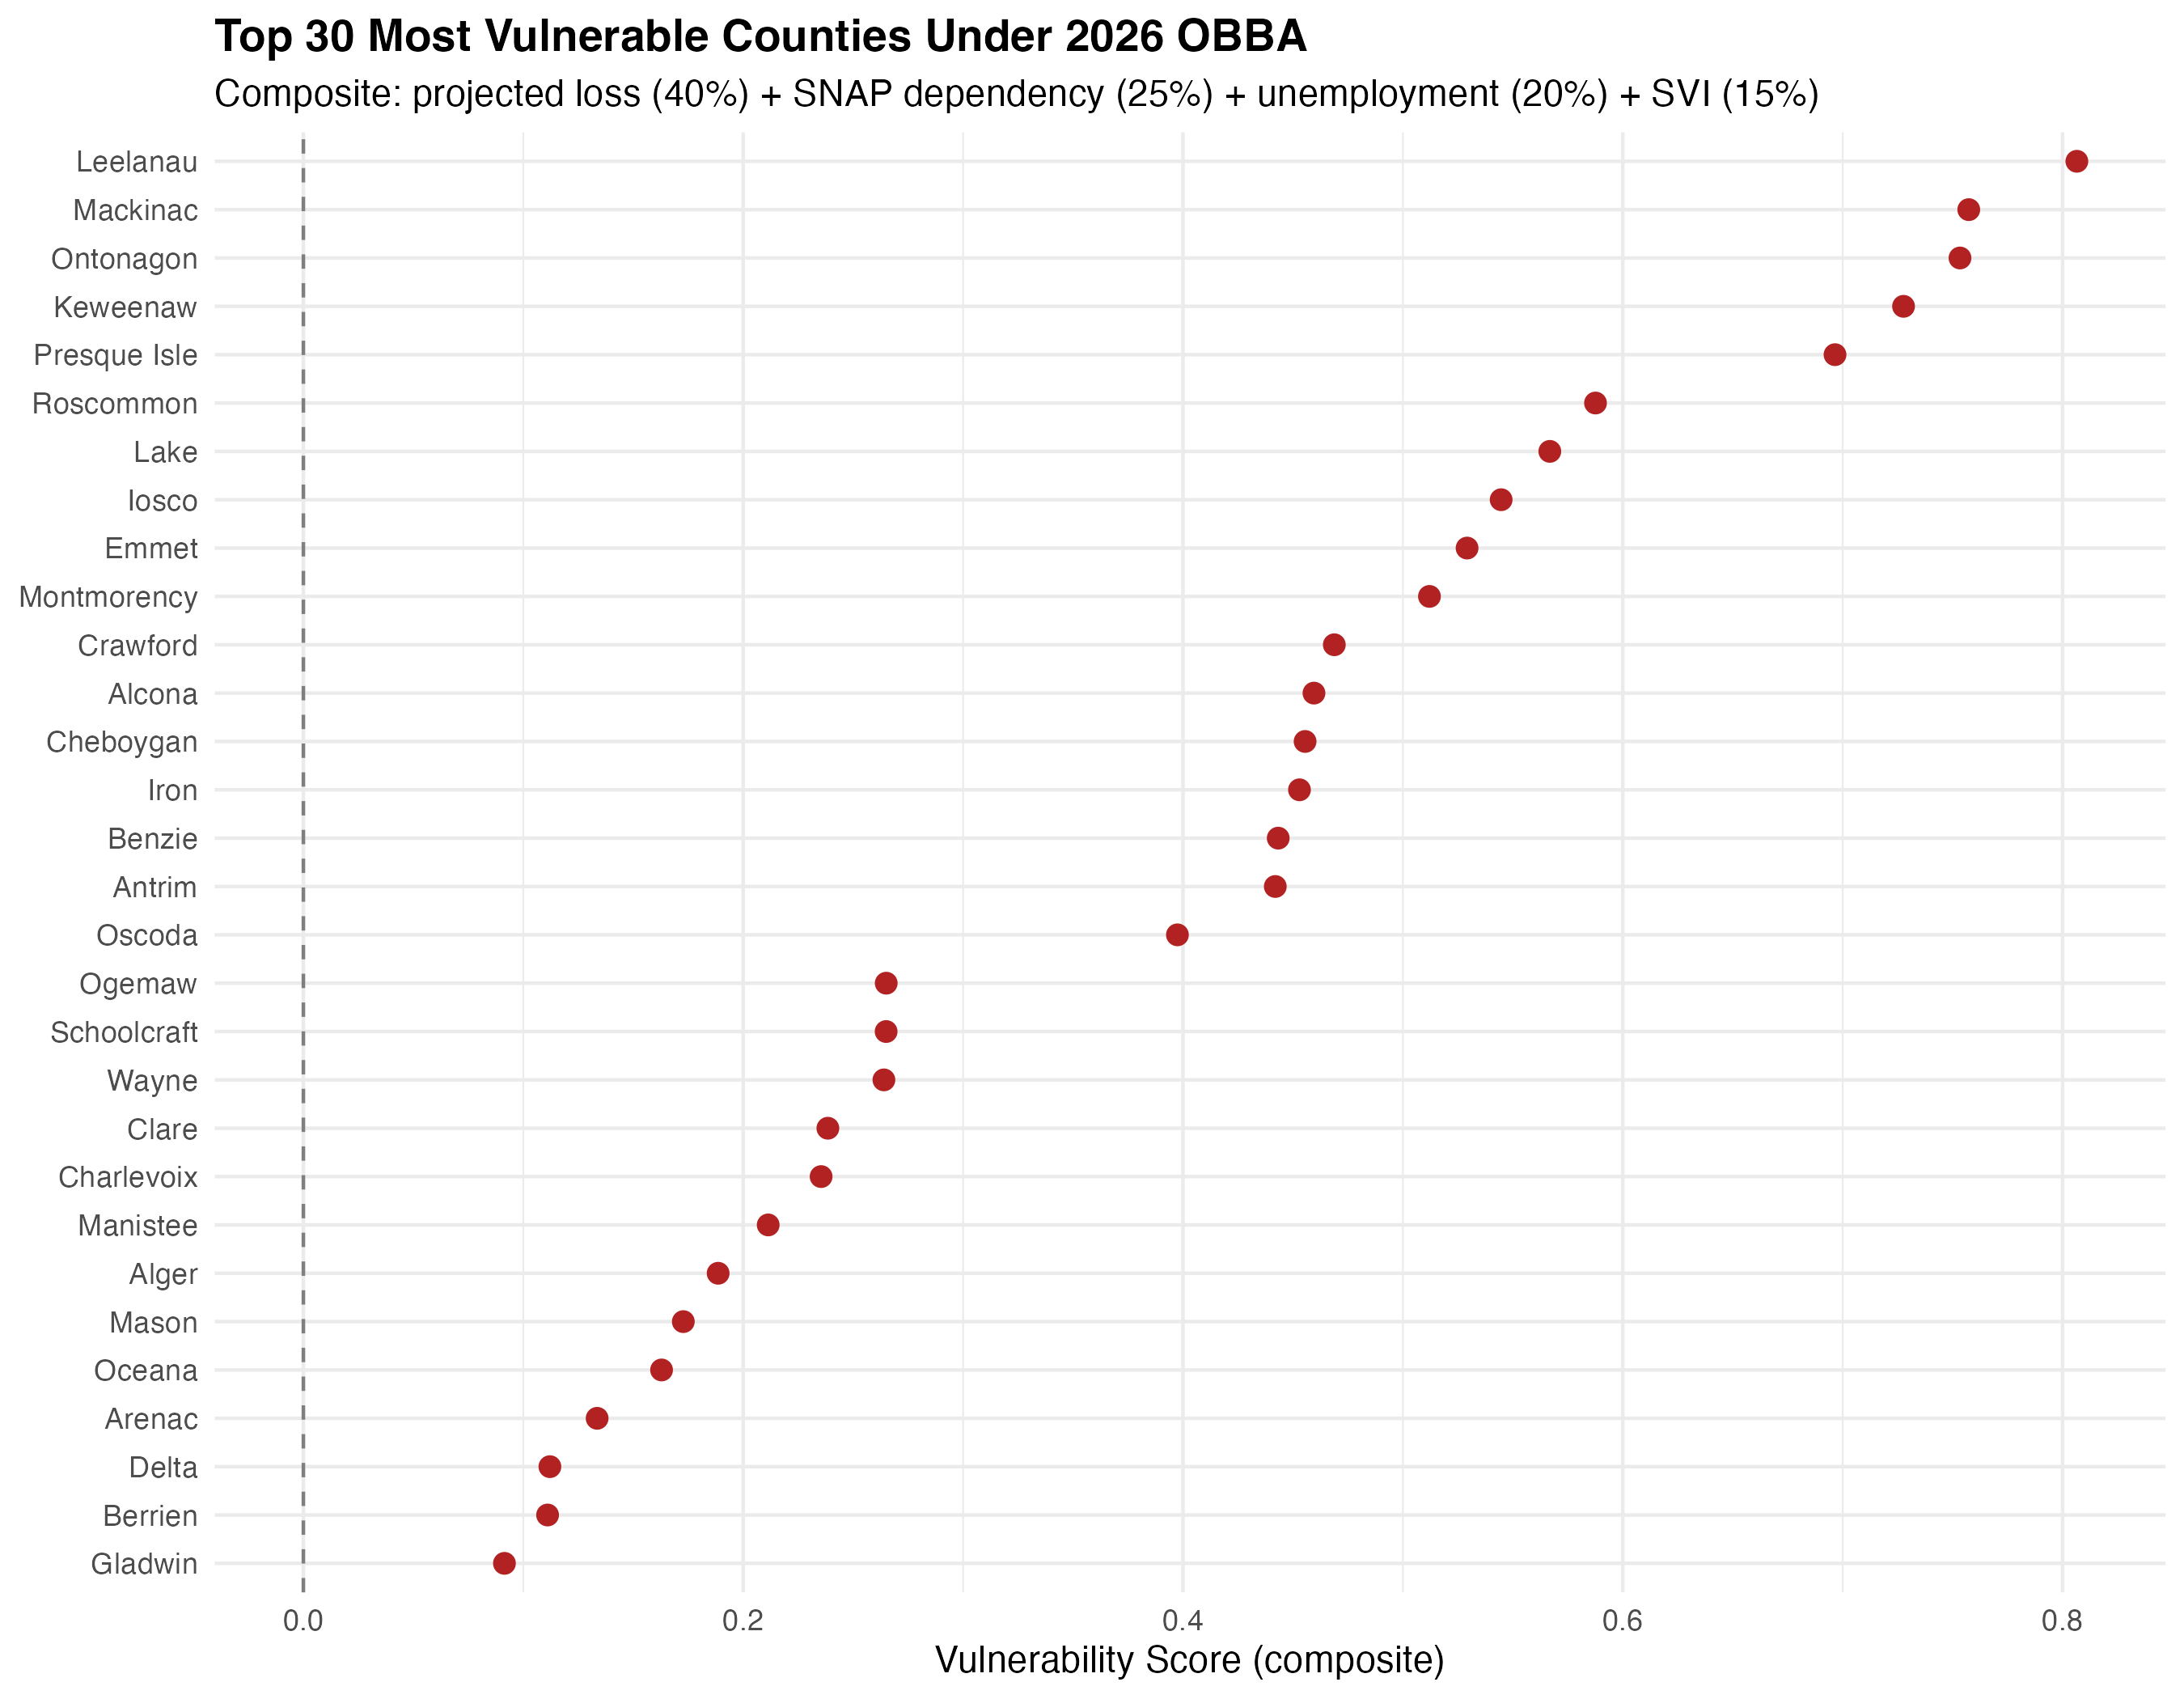
\includegraphics[width=\textwidth]{../outputs/figures/vulnerability_ranking_dotplot}
\end{column}
\end{columns}

\end{frame}

% ====================================================================
% 10. VULNERABILITY MAP  (~1 min)
% ====================================================================
\begin{frame}{County Vulnerability Map}

\begin{columns}[T]
\begin{column}{0.55\textwidth}
  \centering
  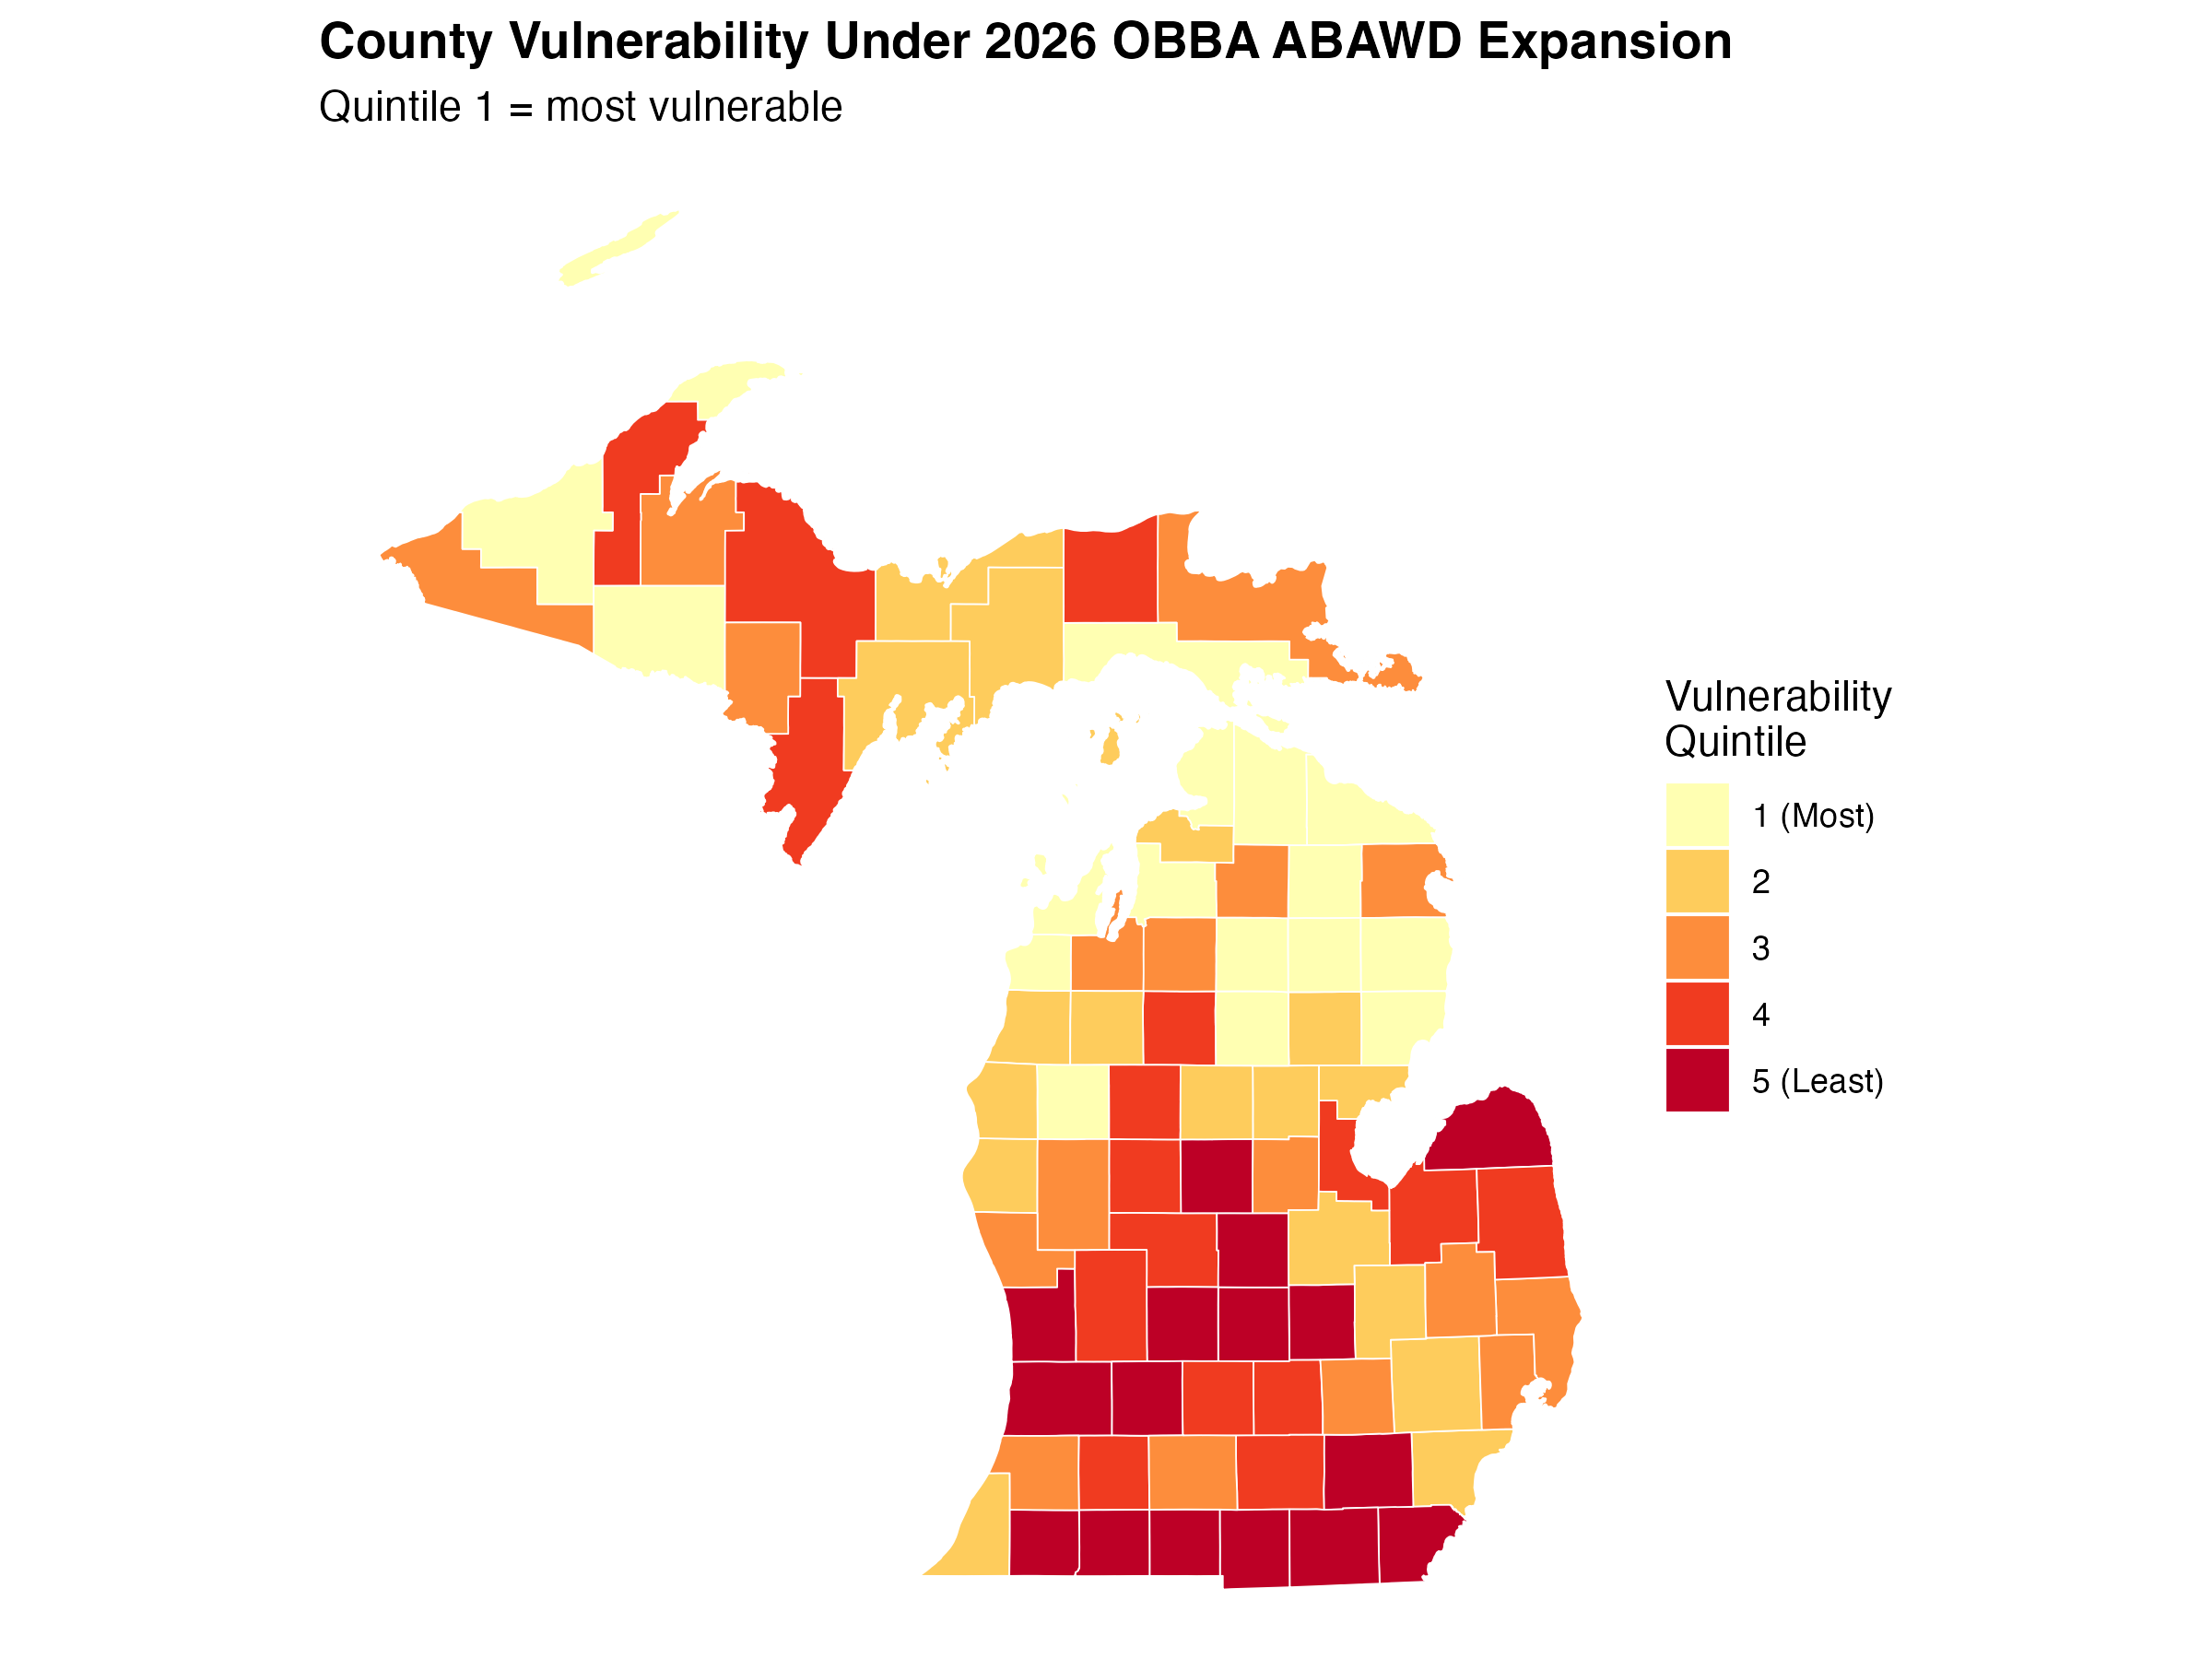
\includegraphics[width=0.95\textwidth]{../outputs/figures/vulnerability_map}
\end{column}
\begin{column}{0.42\textwidth}
  \textbf{Most vulnerable:}
  \begin{itemize}
    \item Northern Lower Michigan
    \item Upper Peninsula
    \item High baseline SNAP + moderate education
  \end{itemize}

  \vspace{0.5em}
  \textbf{Least vulnerable:}
  \begin{itemize}
    \item SE Michigan metro
    \item Strong labor markets + service infrastructure
  \end{itemize}

  \vspace{0.5em}
  {\footnotesize Rank uncertainty: median width = 12 positions (bootstrap)}
\end{column}
\end{columns}

\end{frame}

% ====================================================================
% 11. AUTOMATIC STABILIZER  (~1 min)
% ====================================================================
\begin{frame}{SNAP as Automatic Stabilizer}

\begin{columns}[T]
\begin{column}{0.55\textwidth}
  \centering
  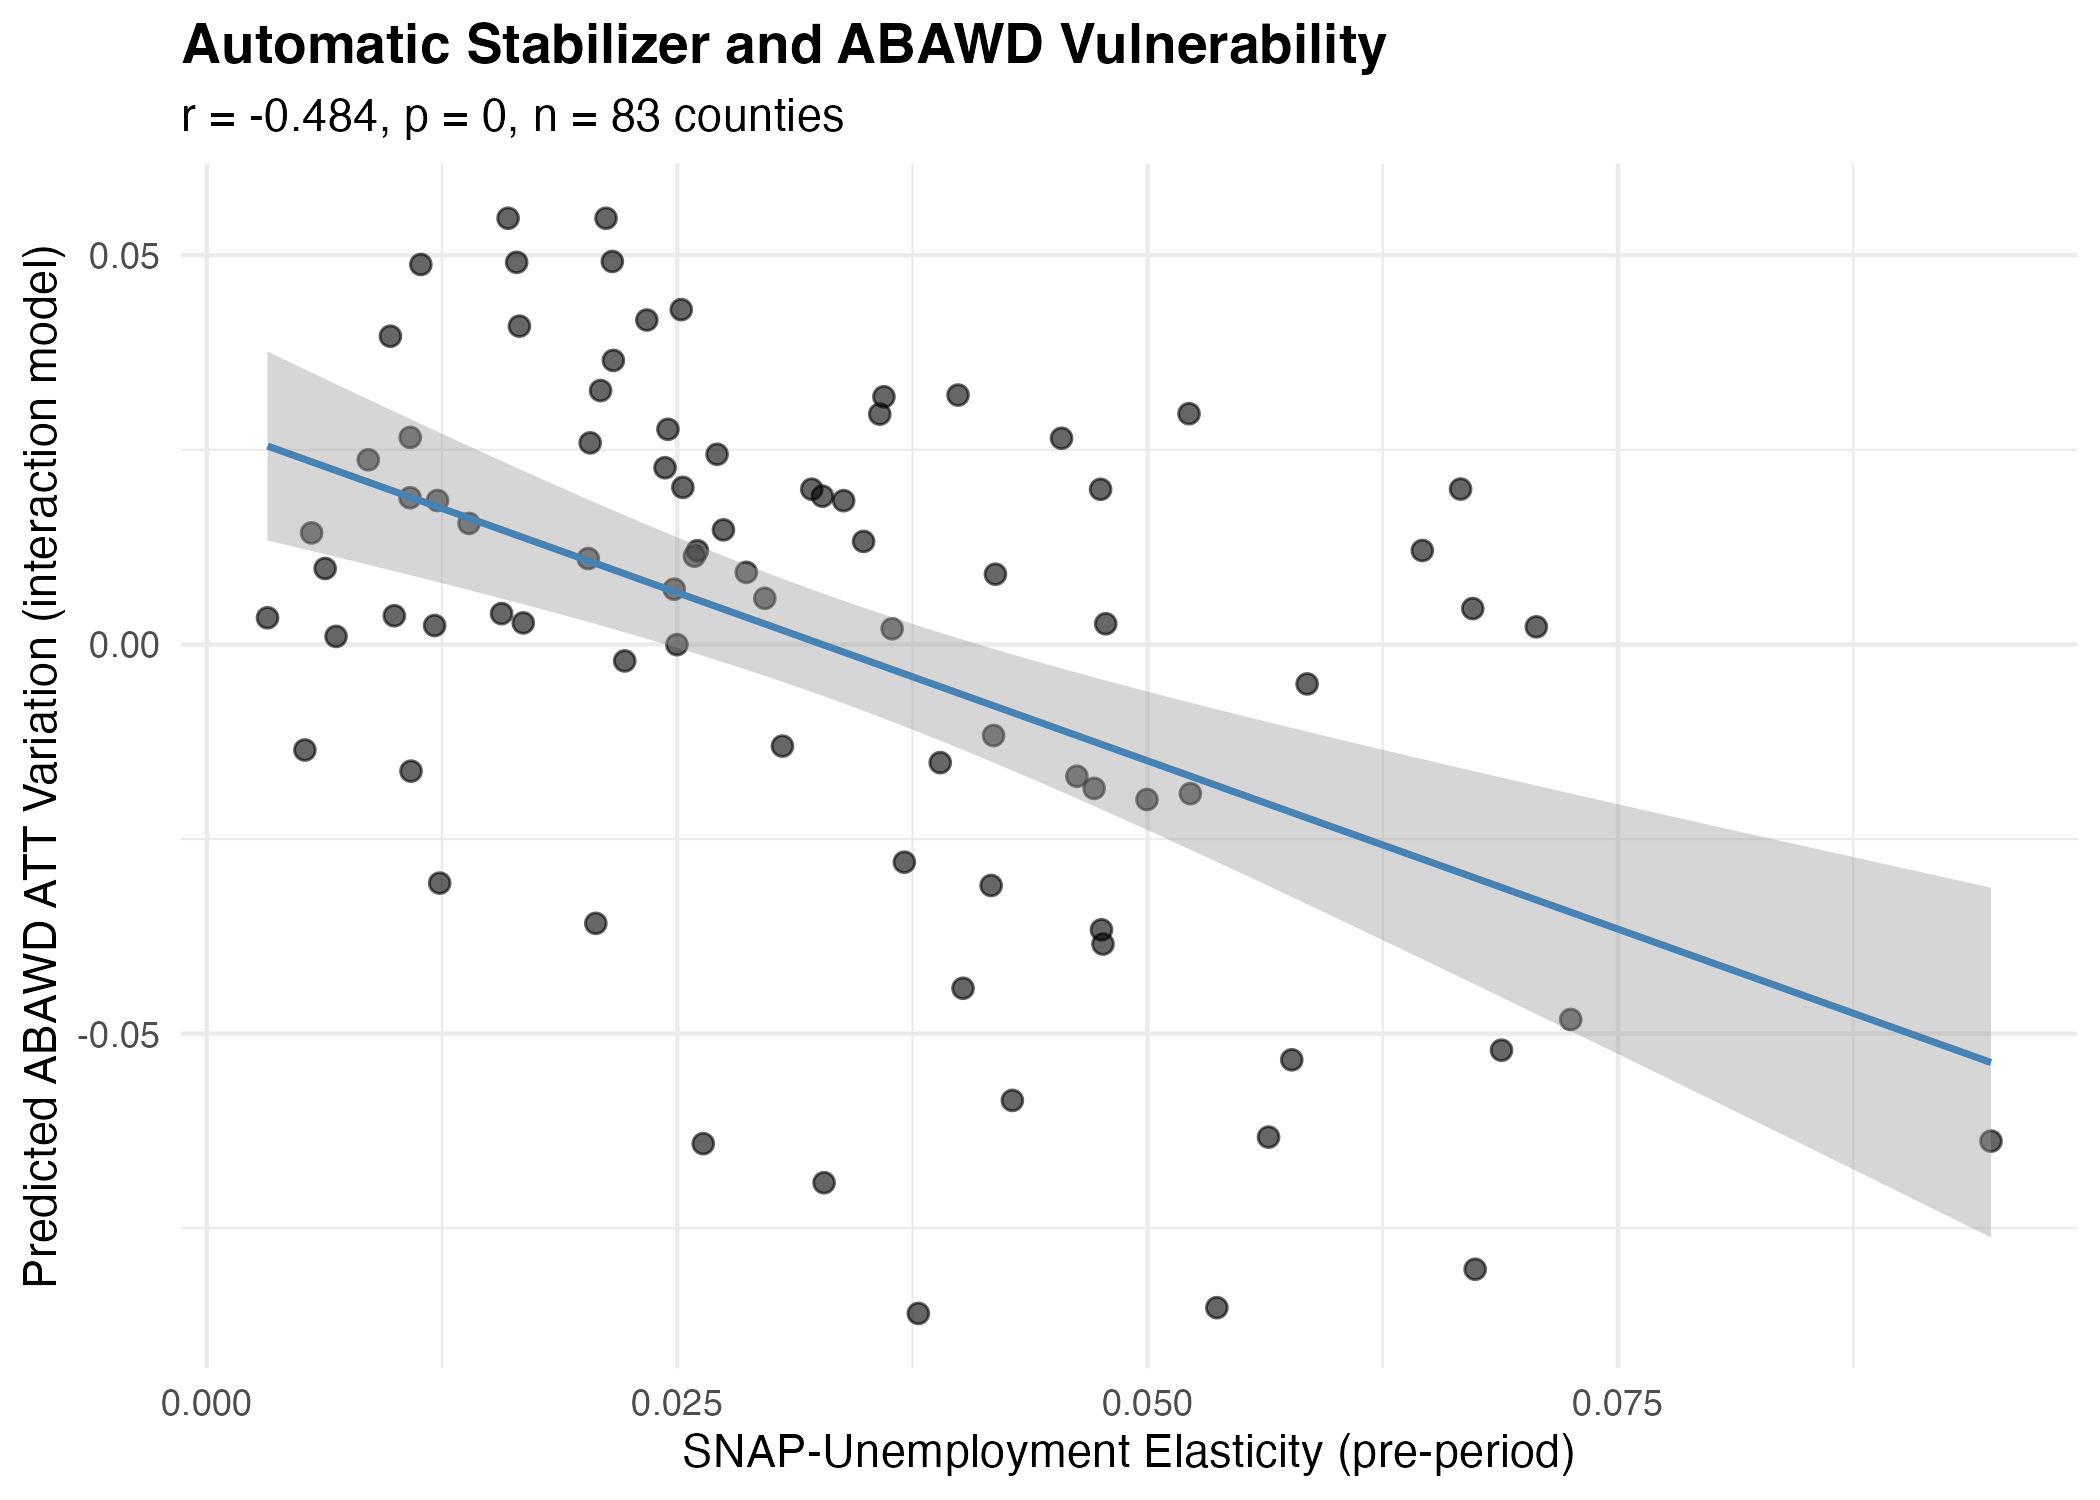
\includegraphics[width=\textwidth]{../outputs/figures/abawd_stabilizer_scatter}
\end{column}
\begin{column}{0.42\textwidth}
  \begin{itemize}
    \item Pre-period: SNAP enrollment rises with unemployment ($\bar{\beta} = 0.033$)
    \item Work requirements \alert{weaken} this stabilizer
    \item $r = -0.48$ ($p < 0.001$): counties where SNAP was most countercyclical $\Rightarrow$ largest participation losses
  \end{itemize}

  \vspace{0.5em}
  {\footnotesize Implication: ABAWD requirements bind hardest where the safety net is most needed}
\end{column}
\end{columns}

\end{frame}

% ====================================================================
% 12. ROBUSTNESS  (~1 min)
% ====================================================================
\begin{frame}{Robustness}

\begin{columns}[T]
\begin{column}{0.55\textwidth}
  \centering
  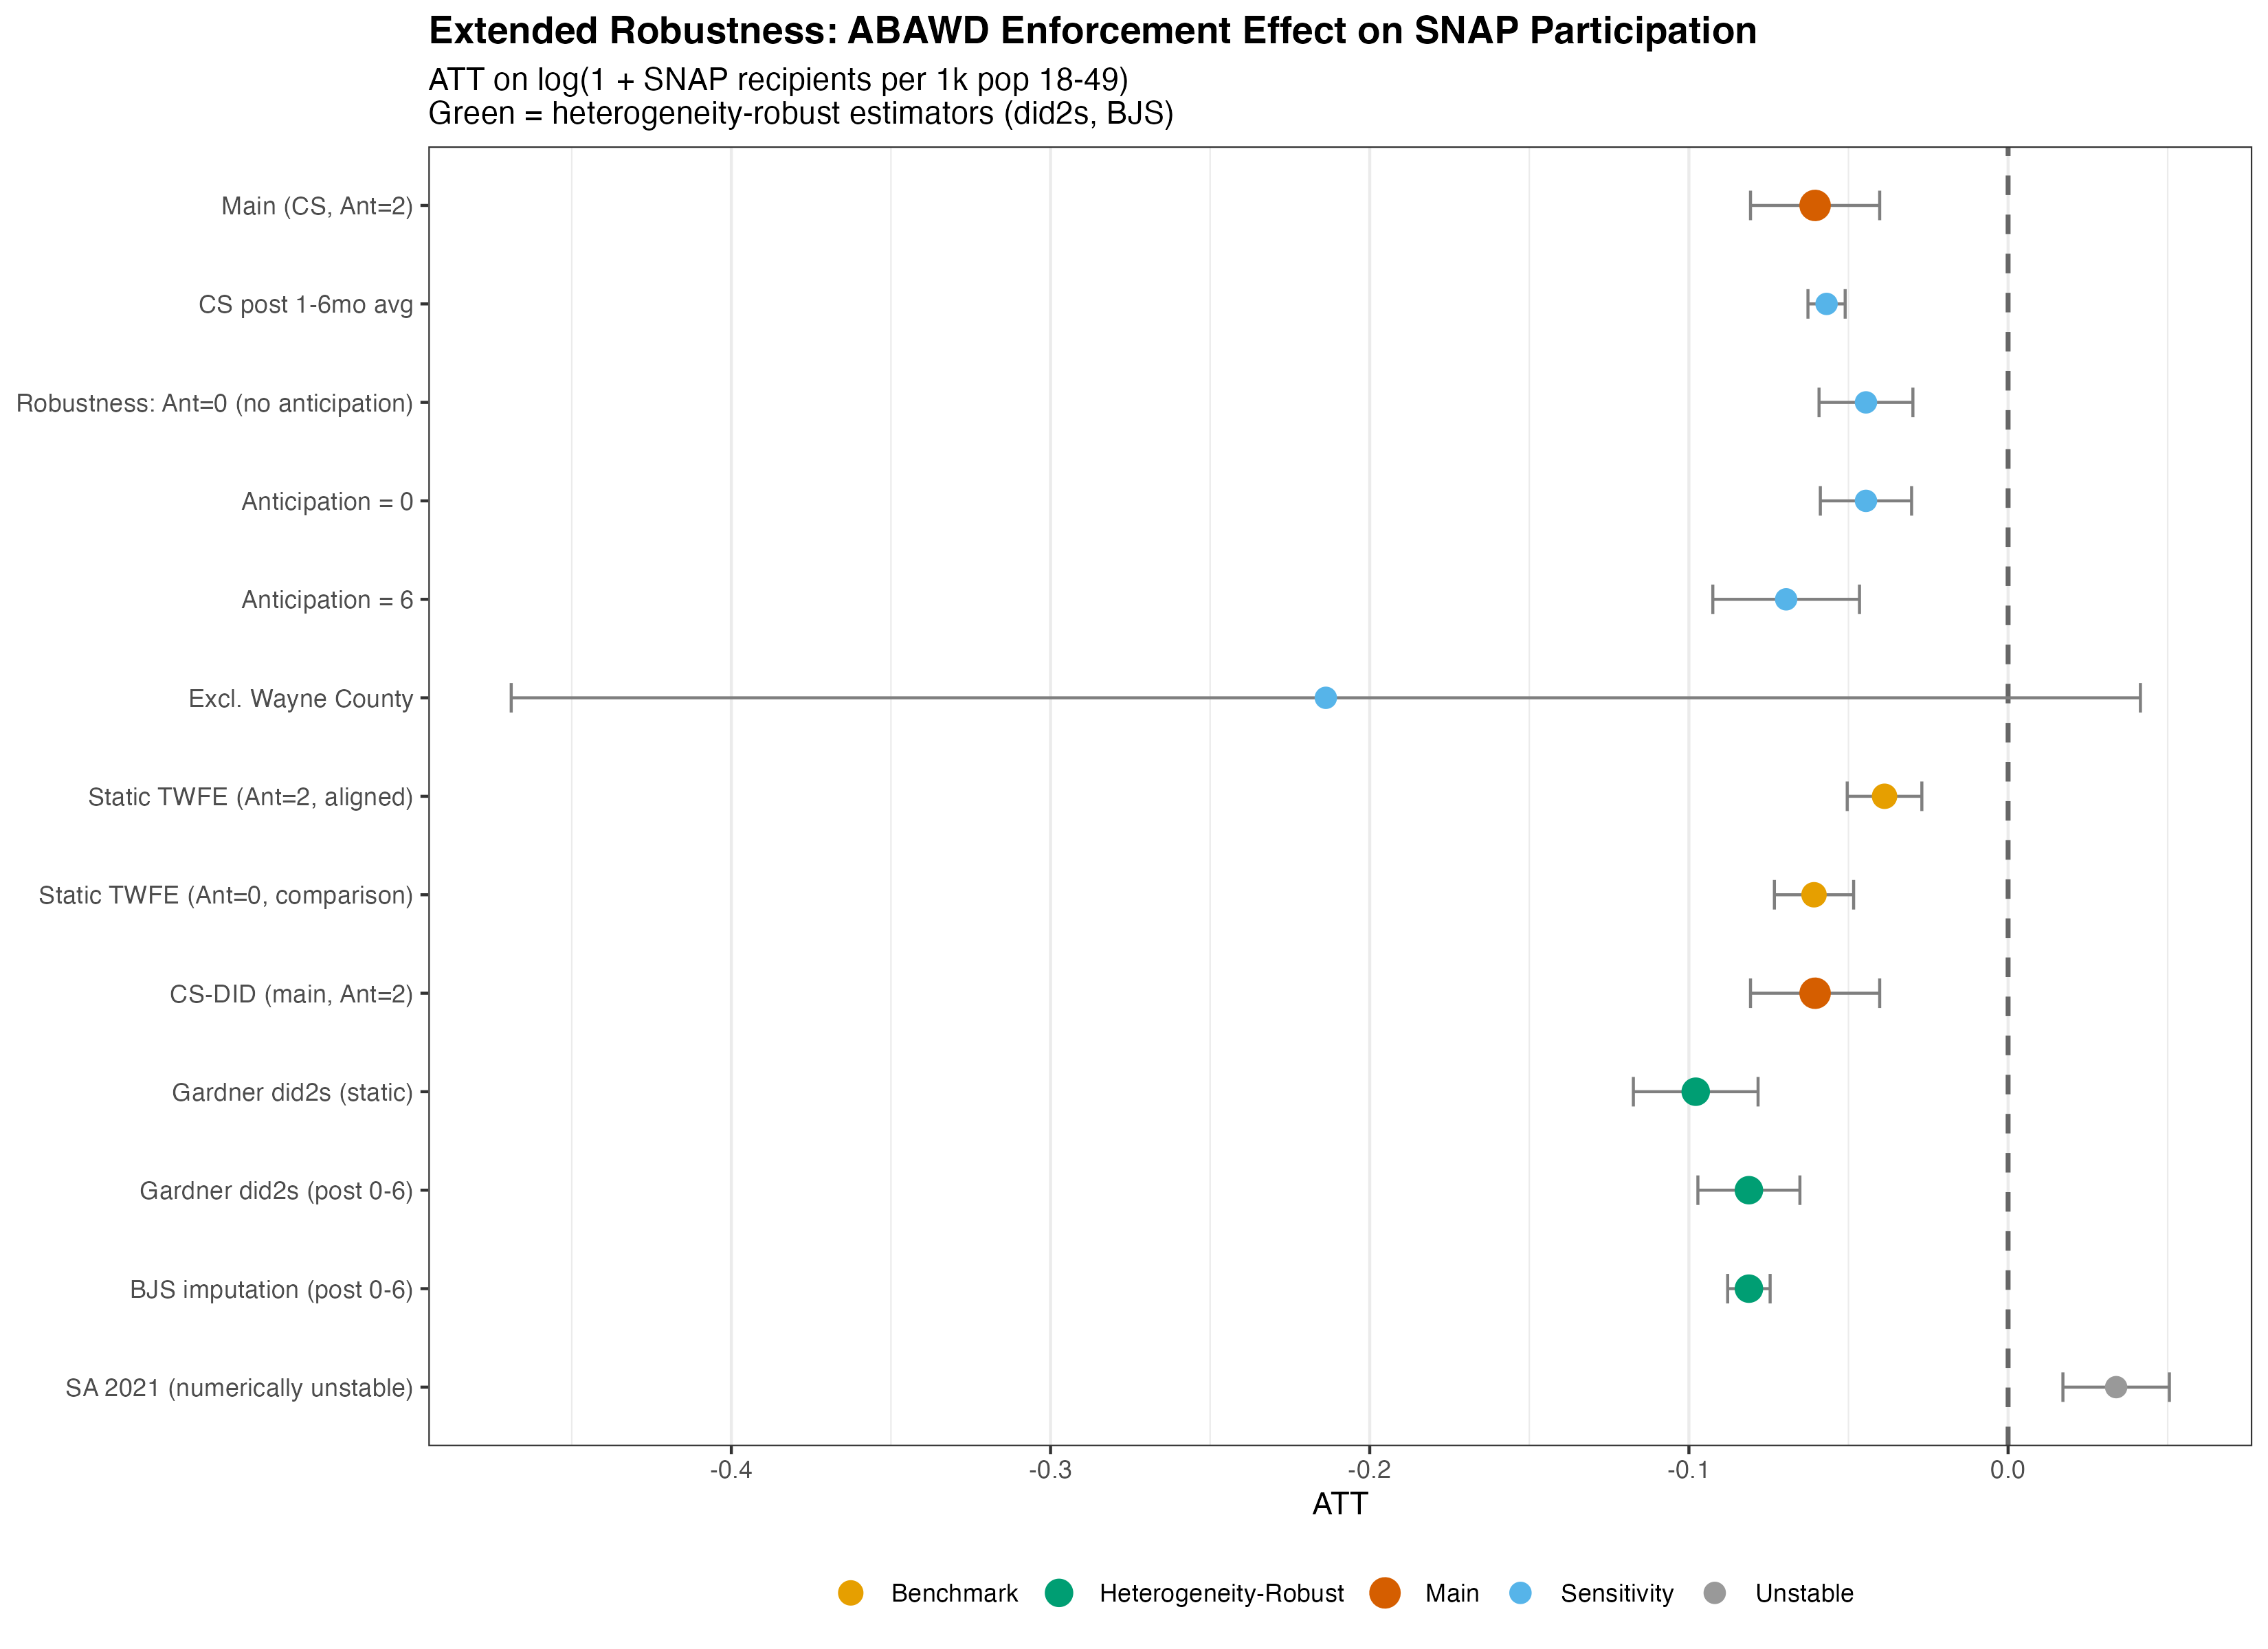
\includegraphics[width=\textwidth]{../outputs/figures/robustness_forest_extended}
\end{column}
\begin{column}{0.42\textwidth}
\small
\textbf{Estimator agreement:}
\begin{itemize}
  \item CS-DID: $-0.060$
  \item did2s: $-0.080$
  \item BJS imputation: $-0.080$
  \item Stacking: $-0.051$
  \item SA: $+0.034$ {\scriptsize (rank deficiency)}
\end{itemize}

\vspace{0.3em}
\textbf{Inference:}
\begin{itemize}
  \item HonestDiD $\bar{M}^* > 2.0$
  \item Fisher permutation $p < 0.002$
  \item Two-way clustering: SE unchanged
\end{itemize}
\end{column}
\end{columns}

\end{frame}

% ====================================================================
% 13. POLICY IMPLICATIONS  (~1 min)
% ====================================================================
\begin{frame}{Policy Implications}

\begin{enumerate}
  \item \textbf{Targeted outreach}: Vulnerability ranking $\Rightarrow$ allocate E\&T slots, case management, and community partnerships by projected need

  \vspace{0.5em}
  \item \textbf{Administrative capacity}: Gradual phase-in $\Rightarrow$ counties need advance staffing for recertification surge

  \vspace{0.5em}
  \item \textbf{Age-specific design}: 55--64 population faces greater compliance barriers (lower LFP, health limitations, retraining barriers) $\Rightarrow$ consider age-adjusted thresholds, expanded medical exemptions

  \vspace{0.5em}
  \item \textbf{Countercyclical concern}: Work requirements weaken SNAP's automatic stabilizer function precisely where it is most needed
\end{enumerate}

\end{frame}

% ====================================================================
% 14. CONCLUSION  (~0.5 min)
% ====================================================================
\begin{frame}{Summary}

\begin{enumerate}
  \item ABAWD enforcement $\Rightarrow$ \textbf{5.8\% reduction} in SNAP participation (gradual, 6-month phase-in)

  \vspace{0.3em}
  \item Heterogeneity by unemployment \& urbanicity is \alert{spurious} (treatment-timing confounding); \textbf{genuine} heterogeneity through education \& poverty

  \vspace{0.3em}
  \item 2026 OBBBA expansion: $\sim$\textbf{10,000} projected losses statewide (CI: 7,200--12,600); concentrated in northern MI \& Upper Peninsula

  \vspace{0.3em}
  \item County vulnerability ranking provides \textbf{actionable tool} for implementation planning
\end{enumerate}

\vspace{0.8em}
\centering
\alert{Thank you!} \quad Questions?

\vspace{0.3em}
{\footnotesize \texttt{zhangji6@msu.edu}}

\end{frame}

% ====================================================================
% APPENDIX SLIDES (backup)
% ====================================================================
\appendix

\begin{frame}[plain]
\centering
\vfill
{\Large \textbf{Backup Slides}}
\vfill
\end{frame}

\begin{frame}{HonestDiD Sensitivity}
  \centering
  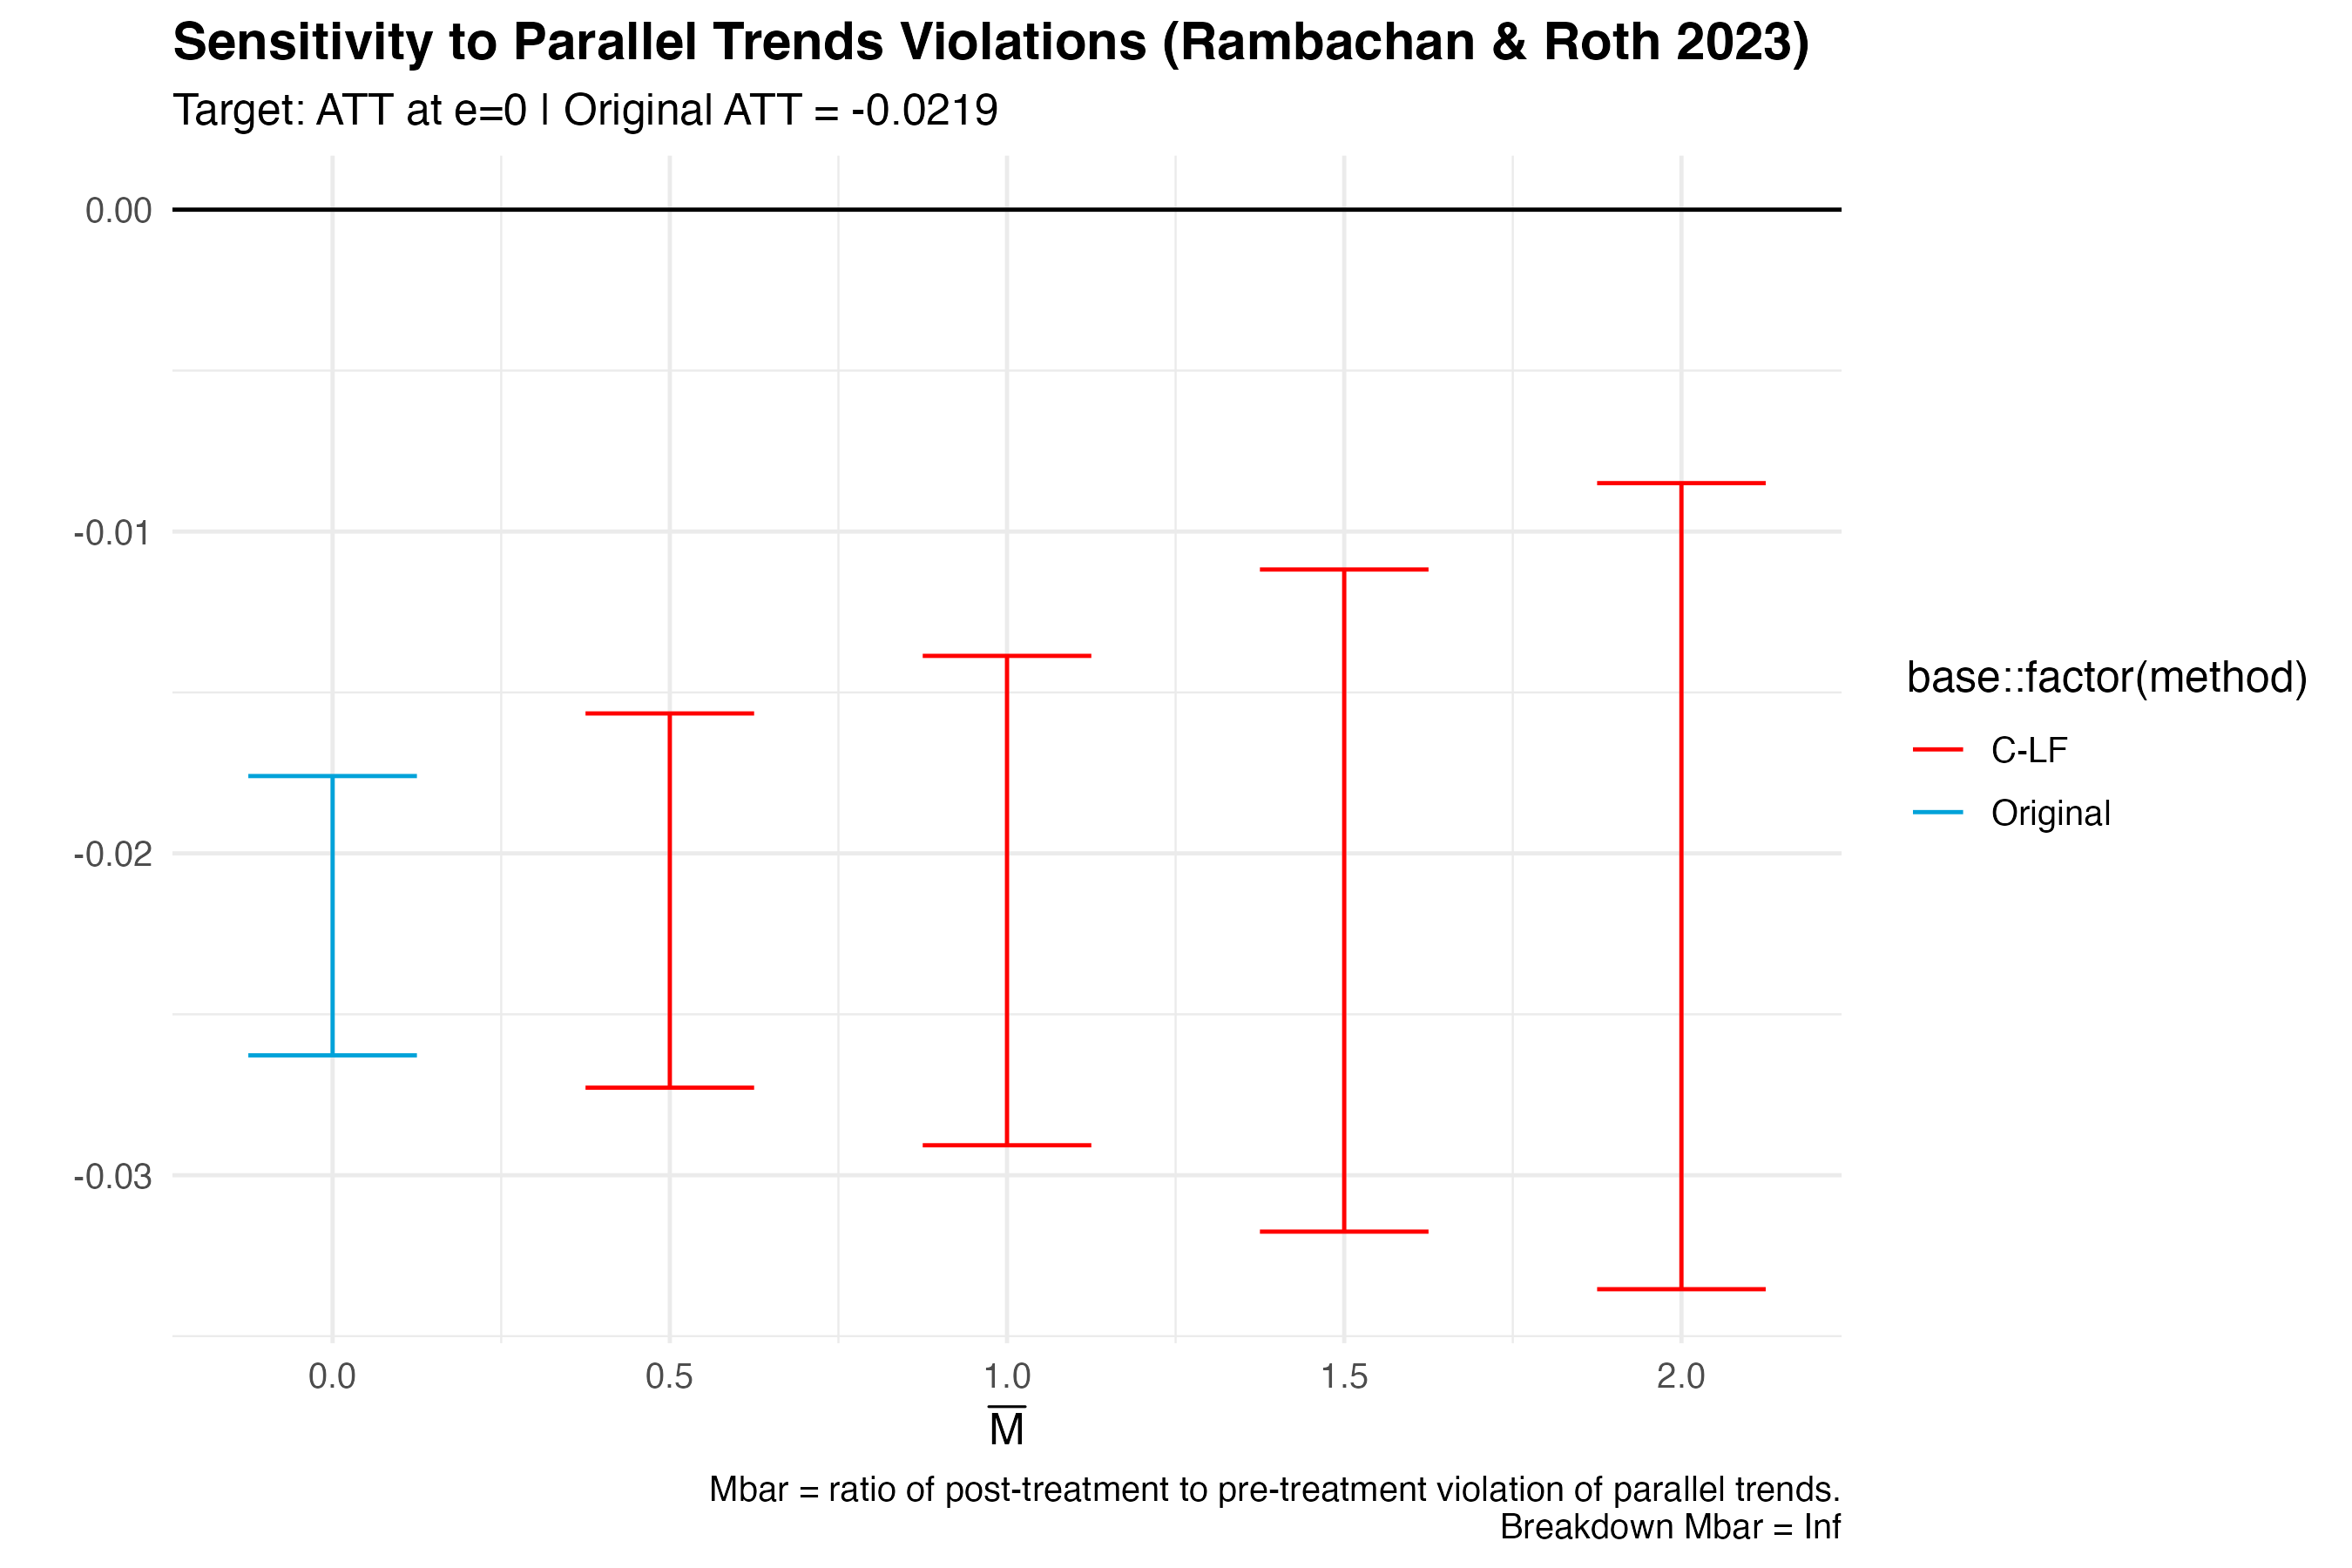
\includegraphics[width=0.45\textwidth]{../outputs/figures/honestdid_sensitivity}
  \hfill
  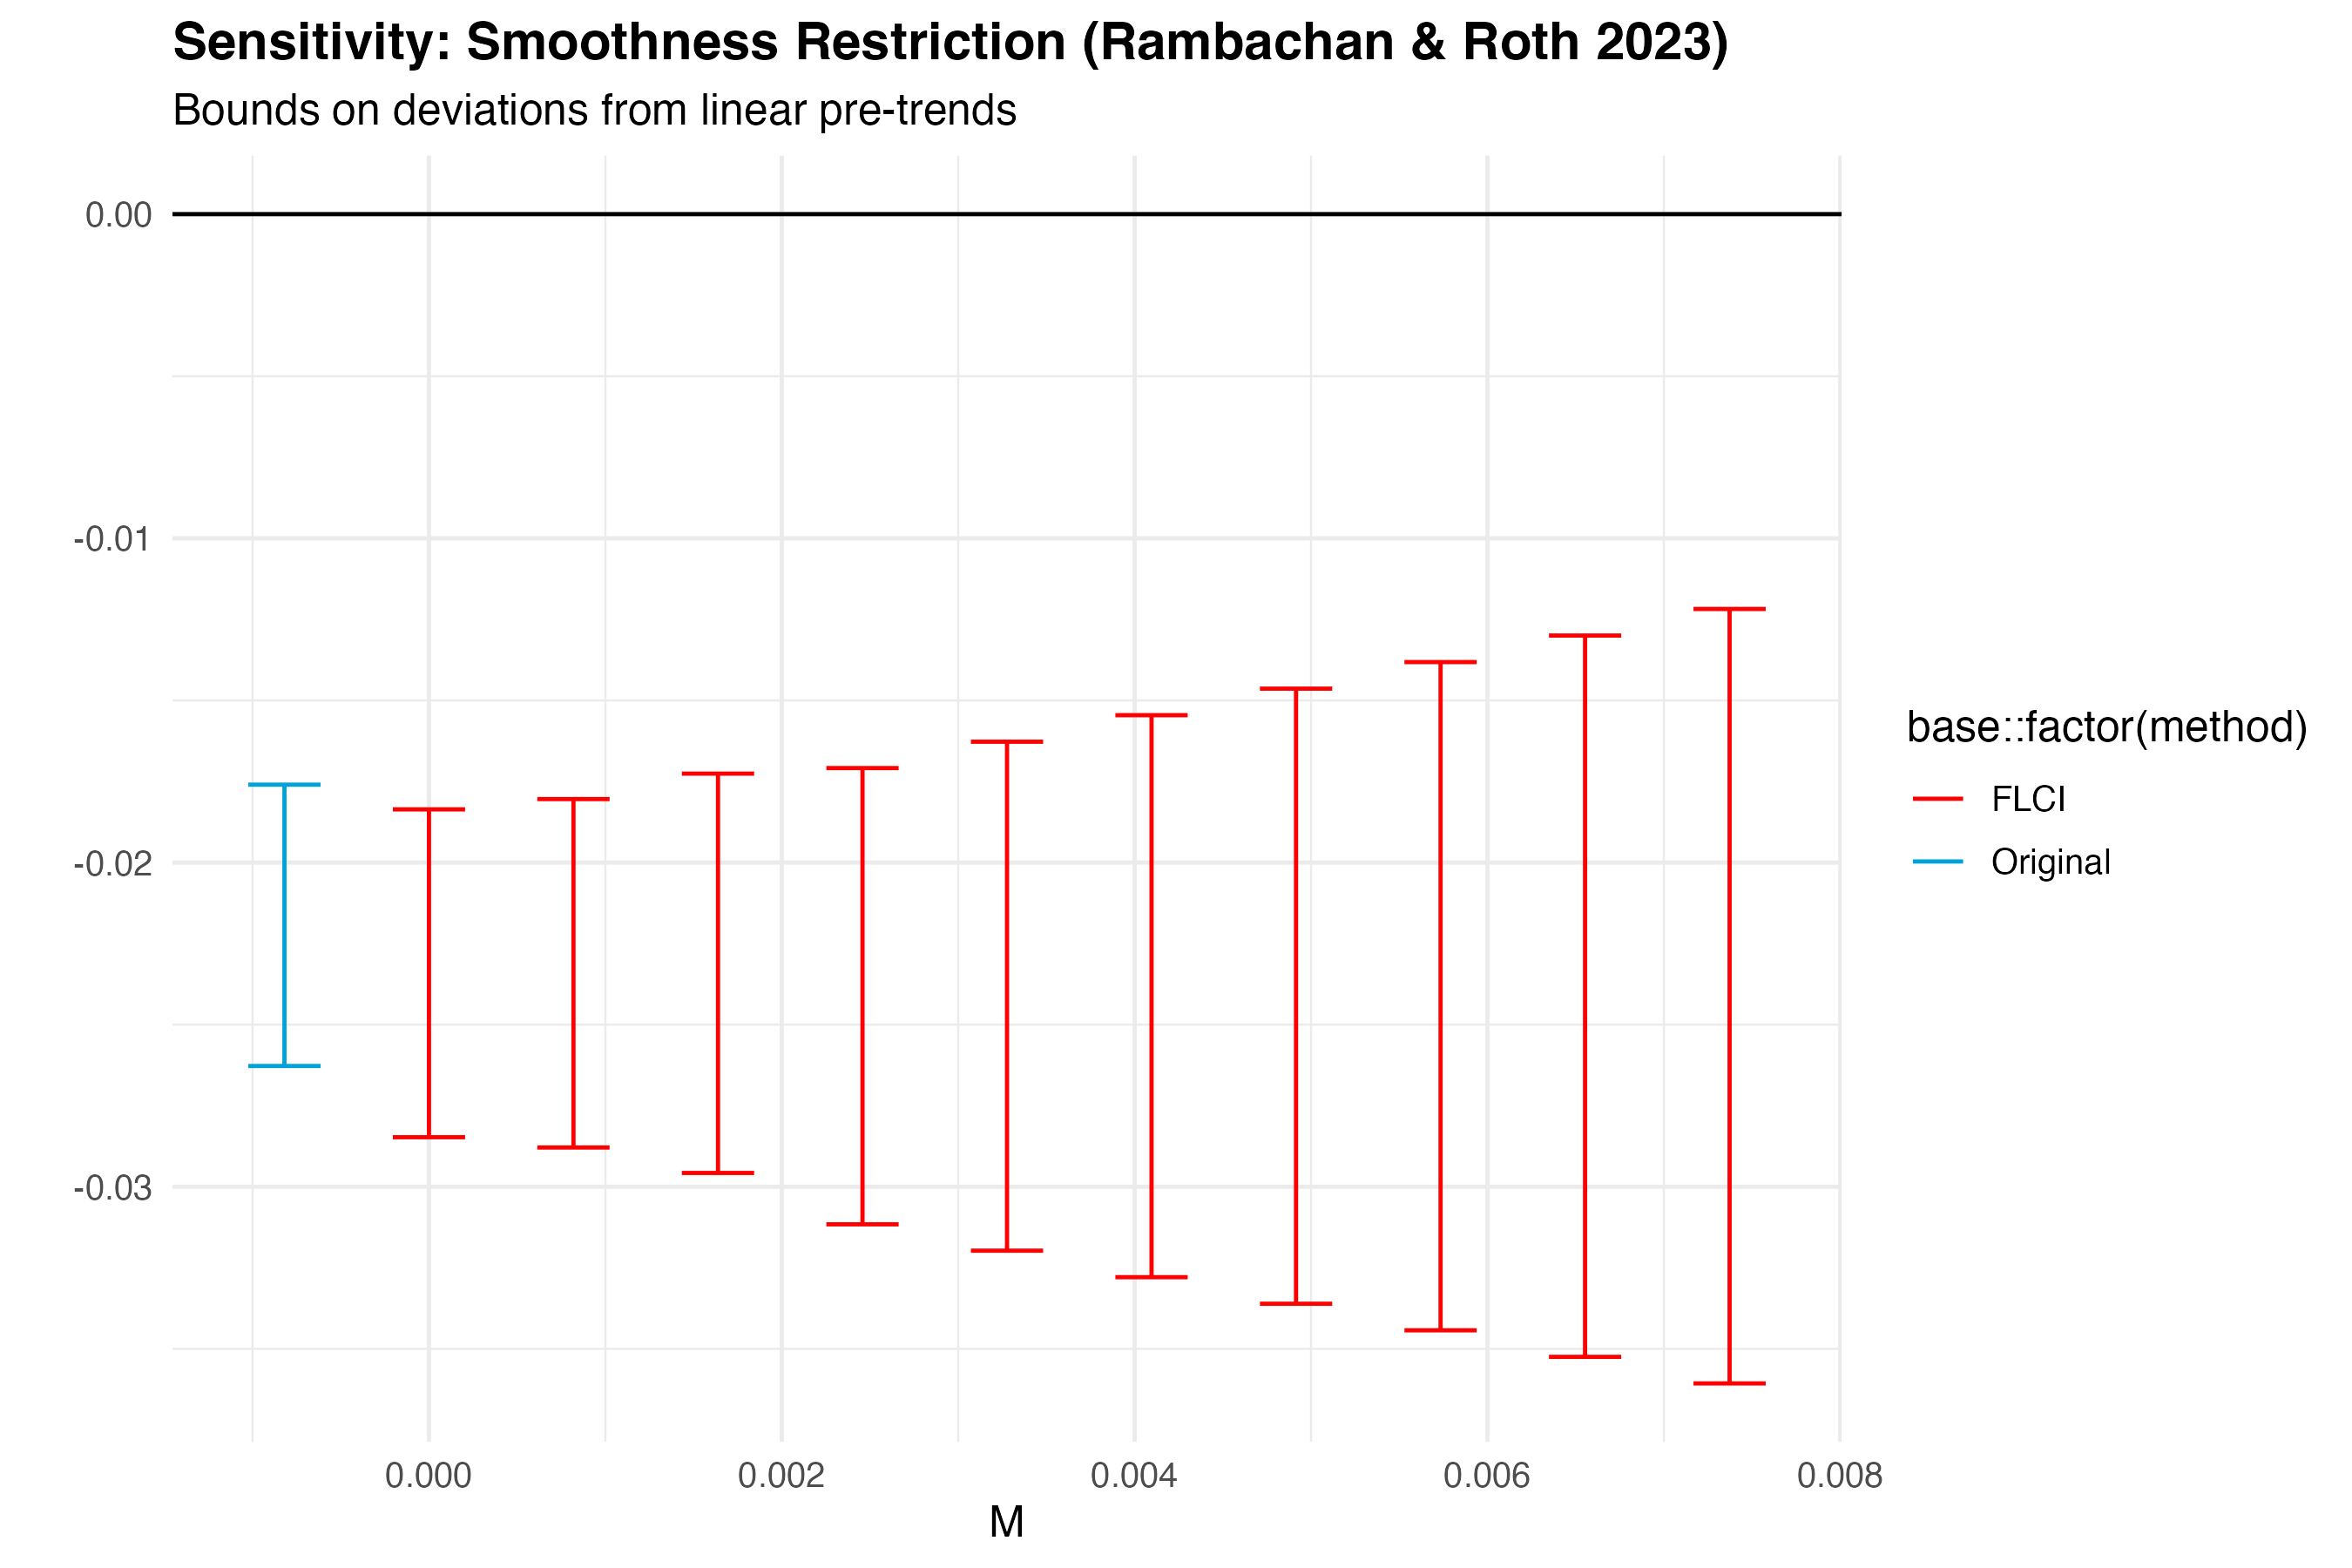
\includegraphics[width=0.45\textwidth]{../outputs/figures/honestdid_smoothness}

  \vspace{0.5em}
  {\small Breakdown value $\bar{M}^* > 2.0$: conclusion holds even if post-treatment violations are 2$\times$ the largest pre-treatment violation.}
\end{frame}

\begin{frame}{Sensitivity of Recession Scenario}
  \centering
  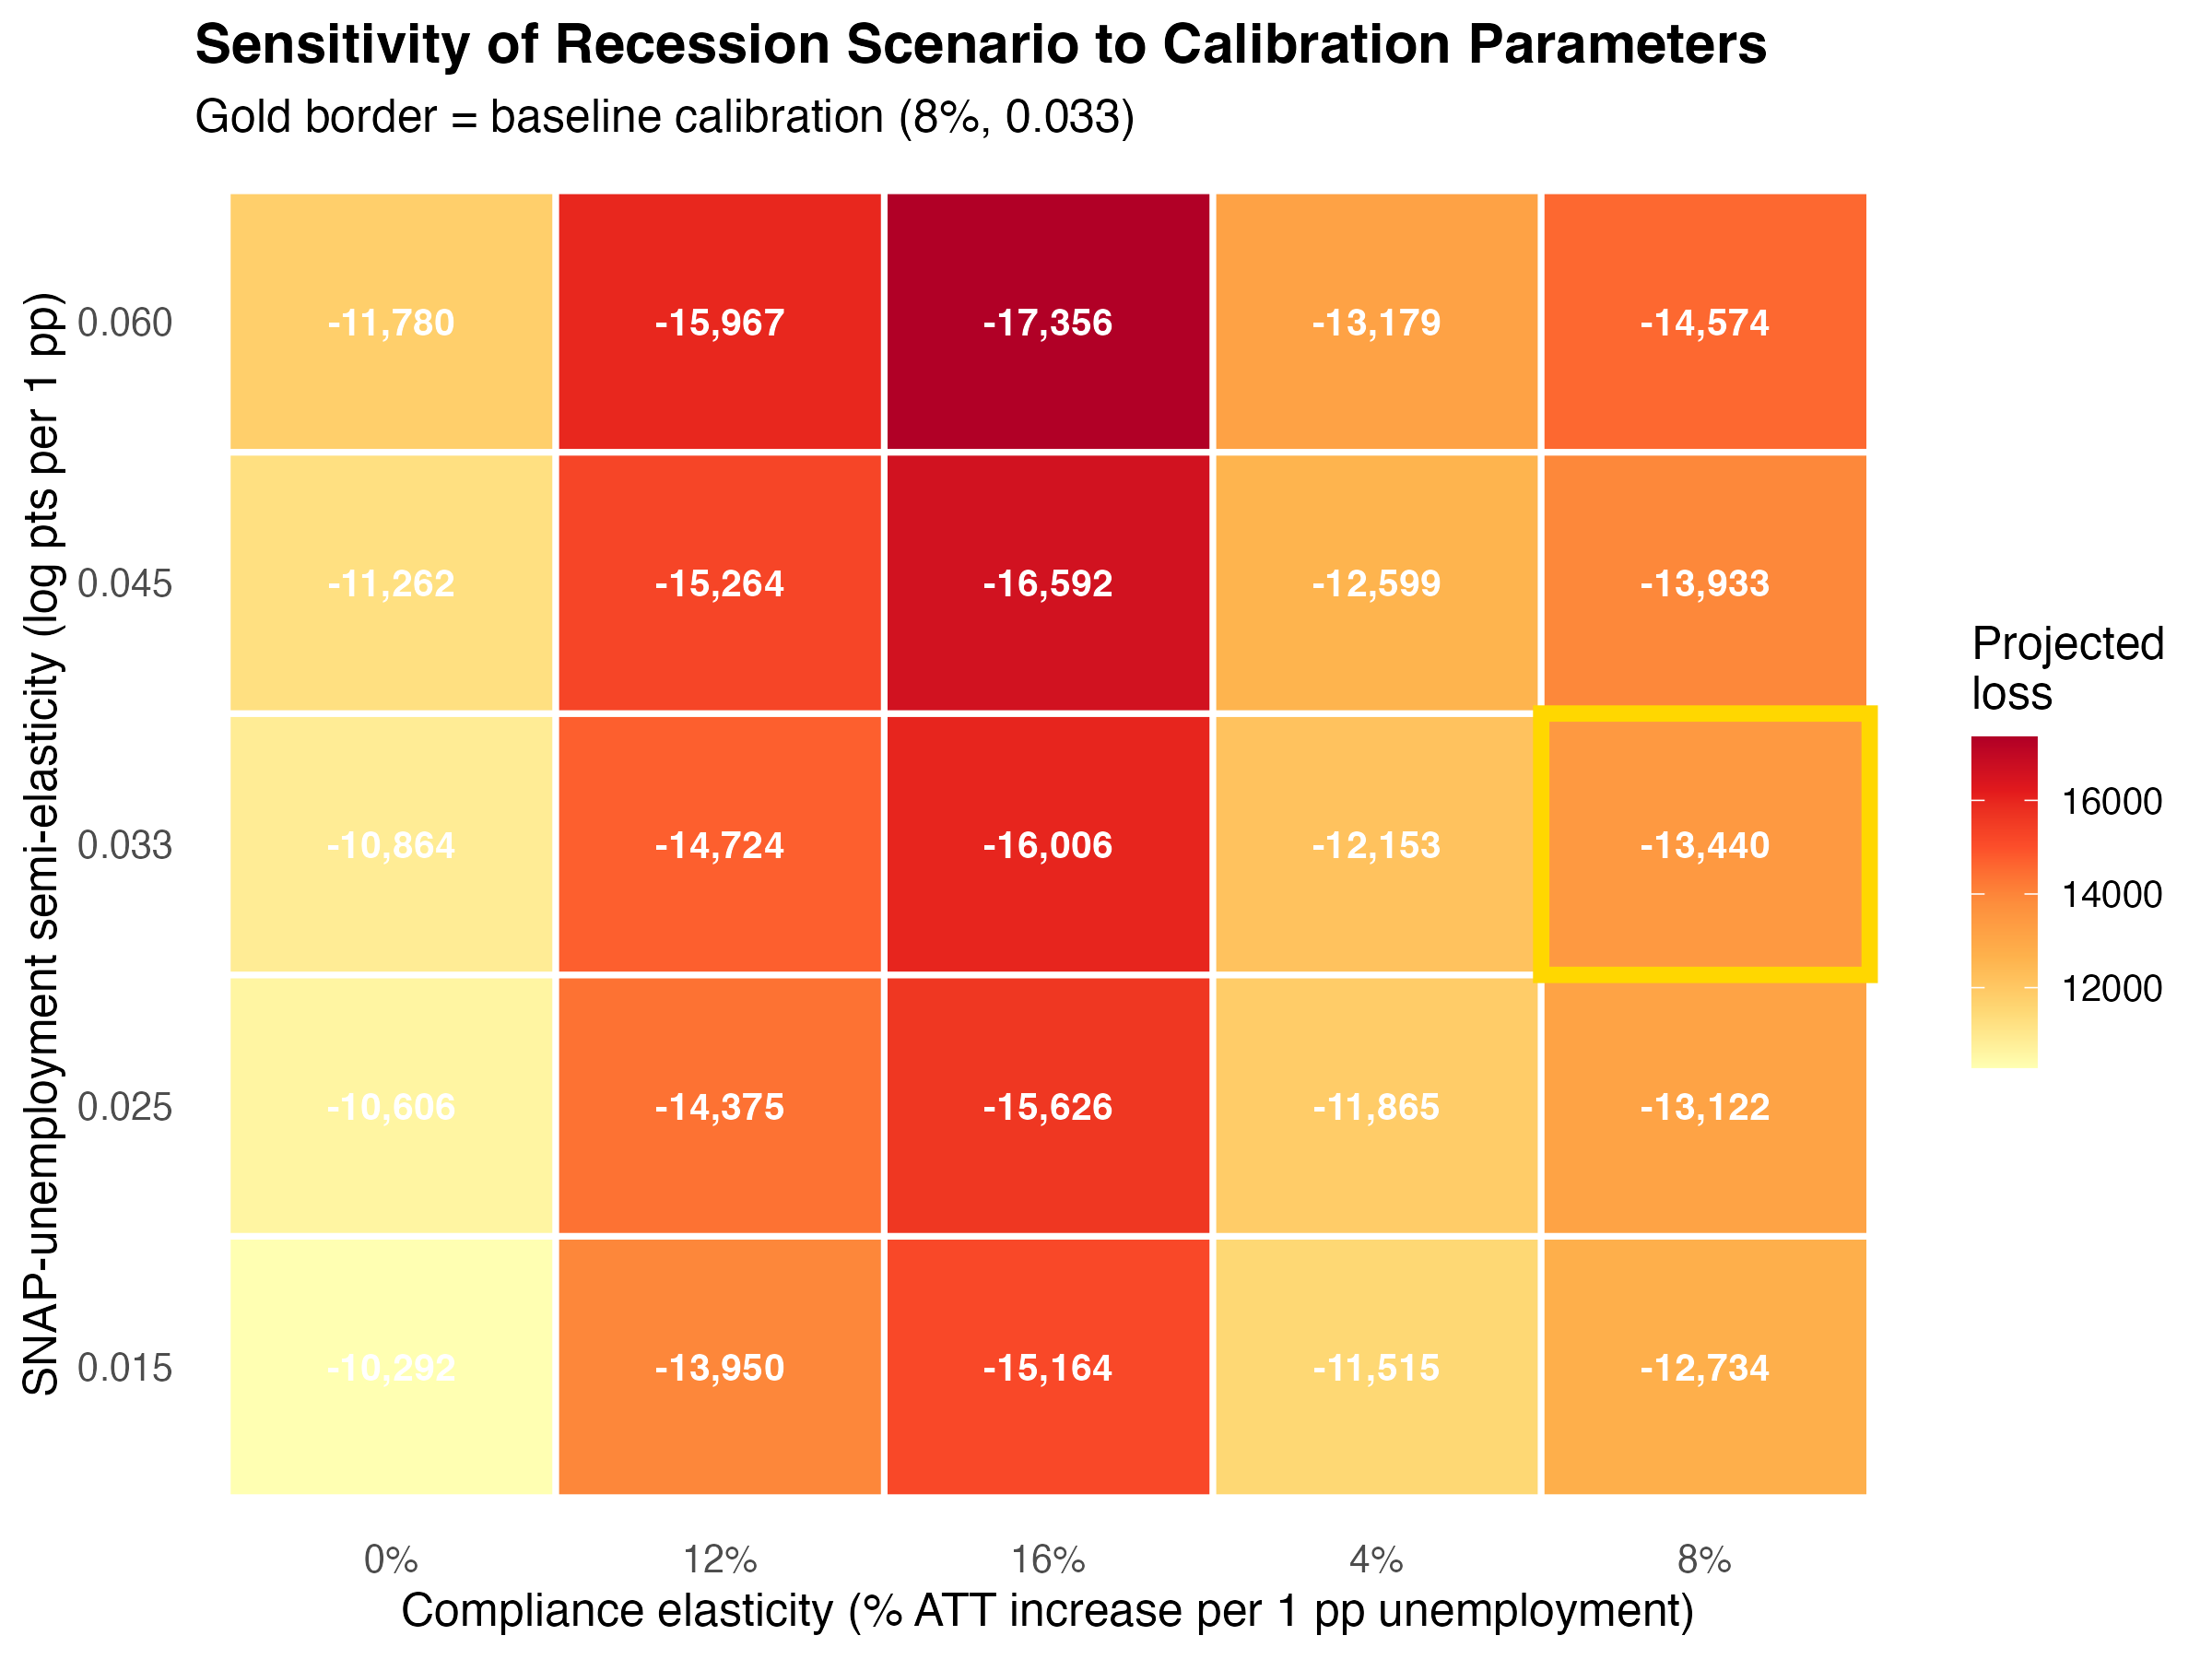
\includegraphics[width=0.55\textwidth]{../outputs/figures/sensitivity_heatmap}

  \vspace{0.2em}
  {\small Gold cell = baseline (8\% compliance elast., 0.033 semi-elast.).  Grid: 10,300--17,400.}
\end{frame}

\begin{frame}{Goodman-Bacon Decomposition}
  \centering
  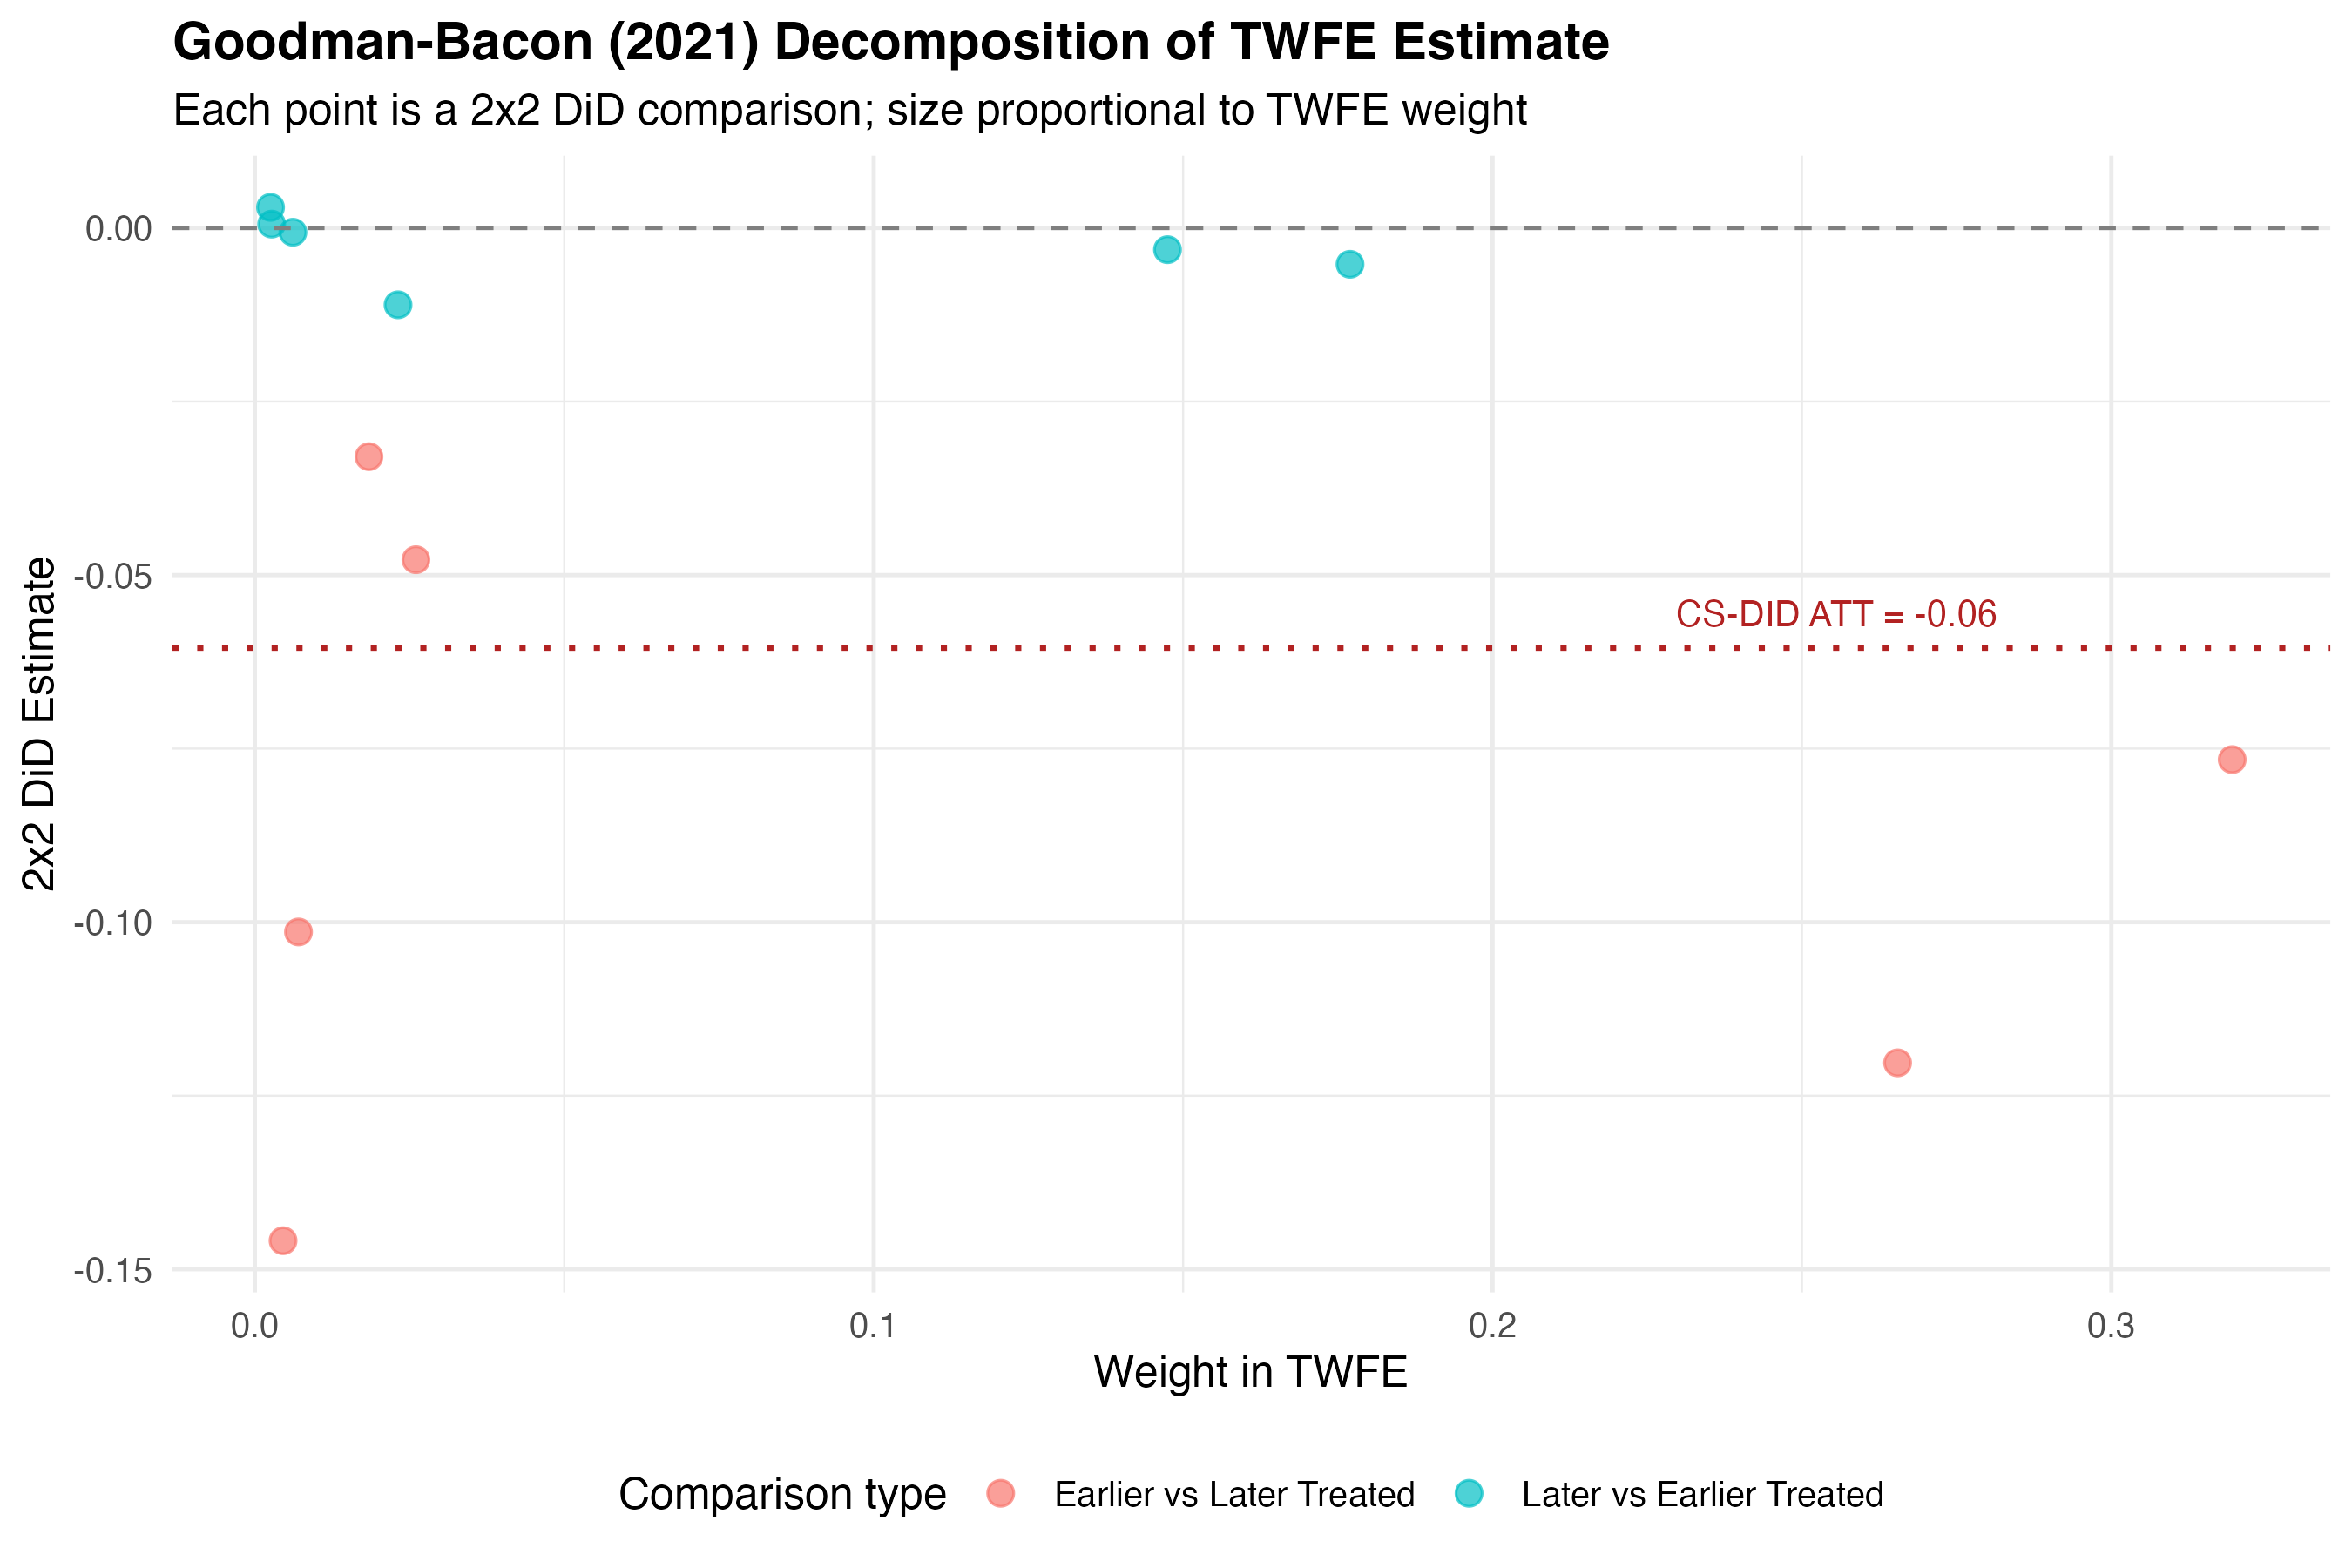
\includegraphics[width=0.65\textwidth]{../outputs/figures/bacon_decomposition}

  \vspace{0.3em}
  {\small Earlier-vs-later (wt=0.64): $-0.093$.  Later-vs-earlier (wt=0.36): $-0.005$.  No sign flip $\Rightarrow$ limited TWFE bias concern.}
\end{frame}

\begin{frame}{Permutation Inference}
  \centering
  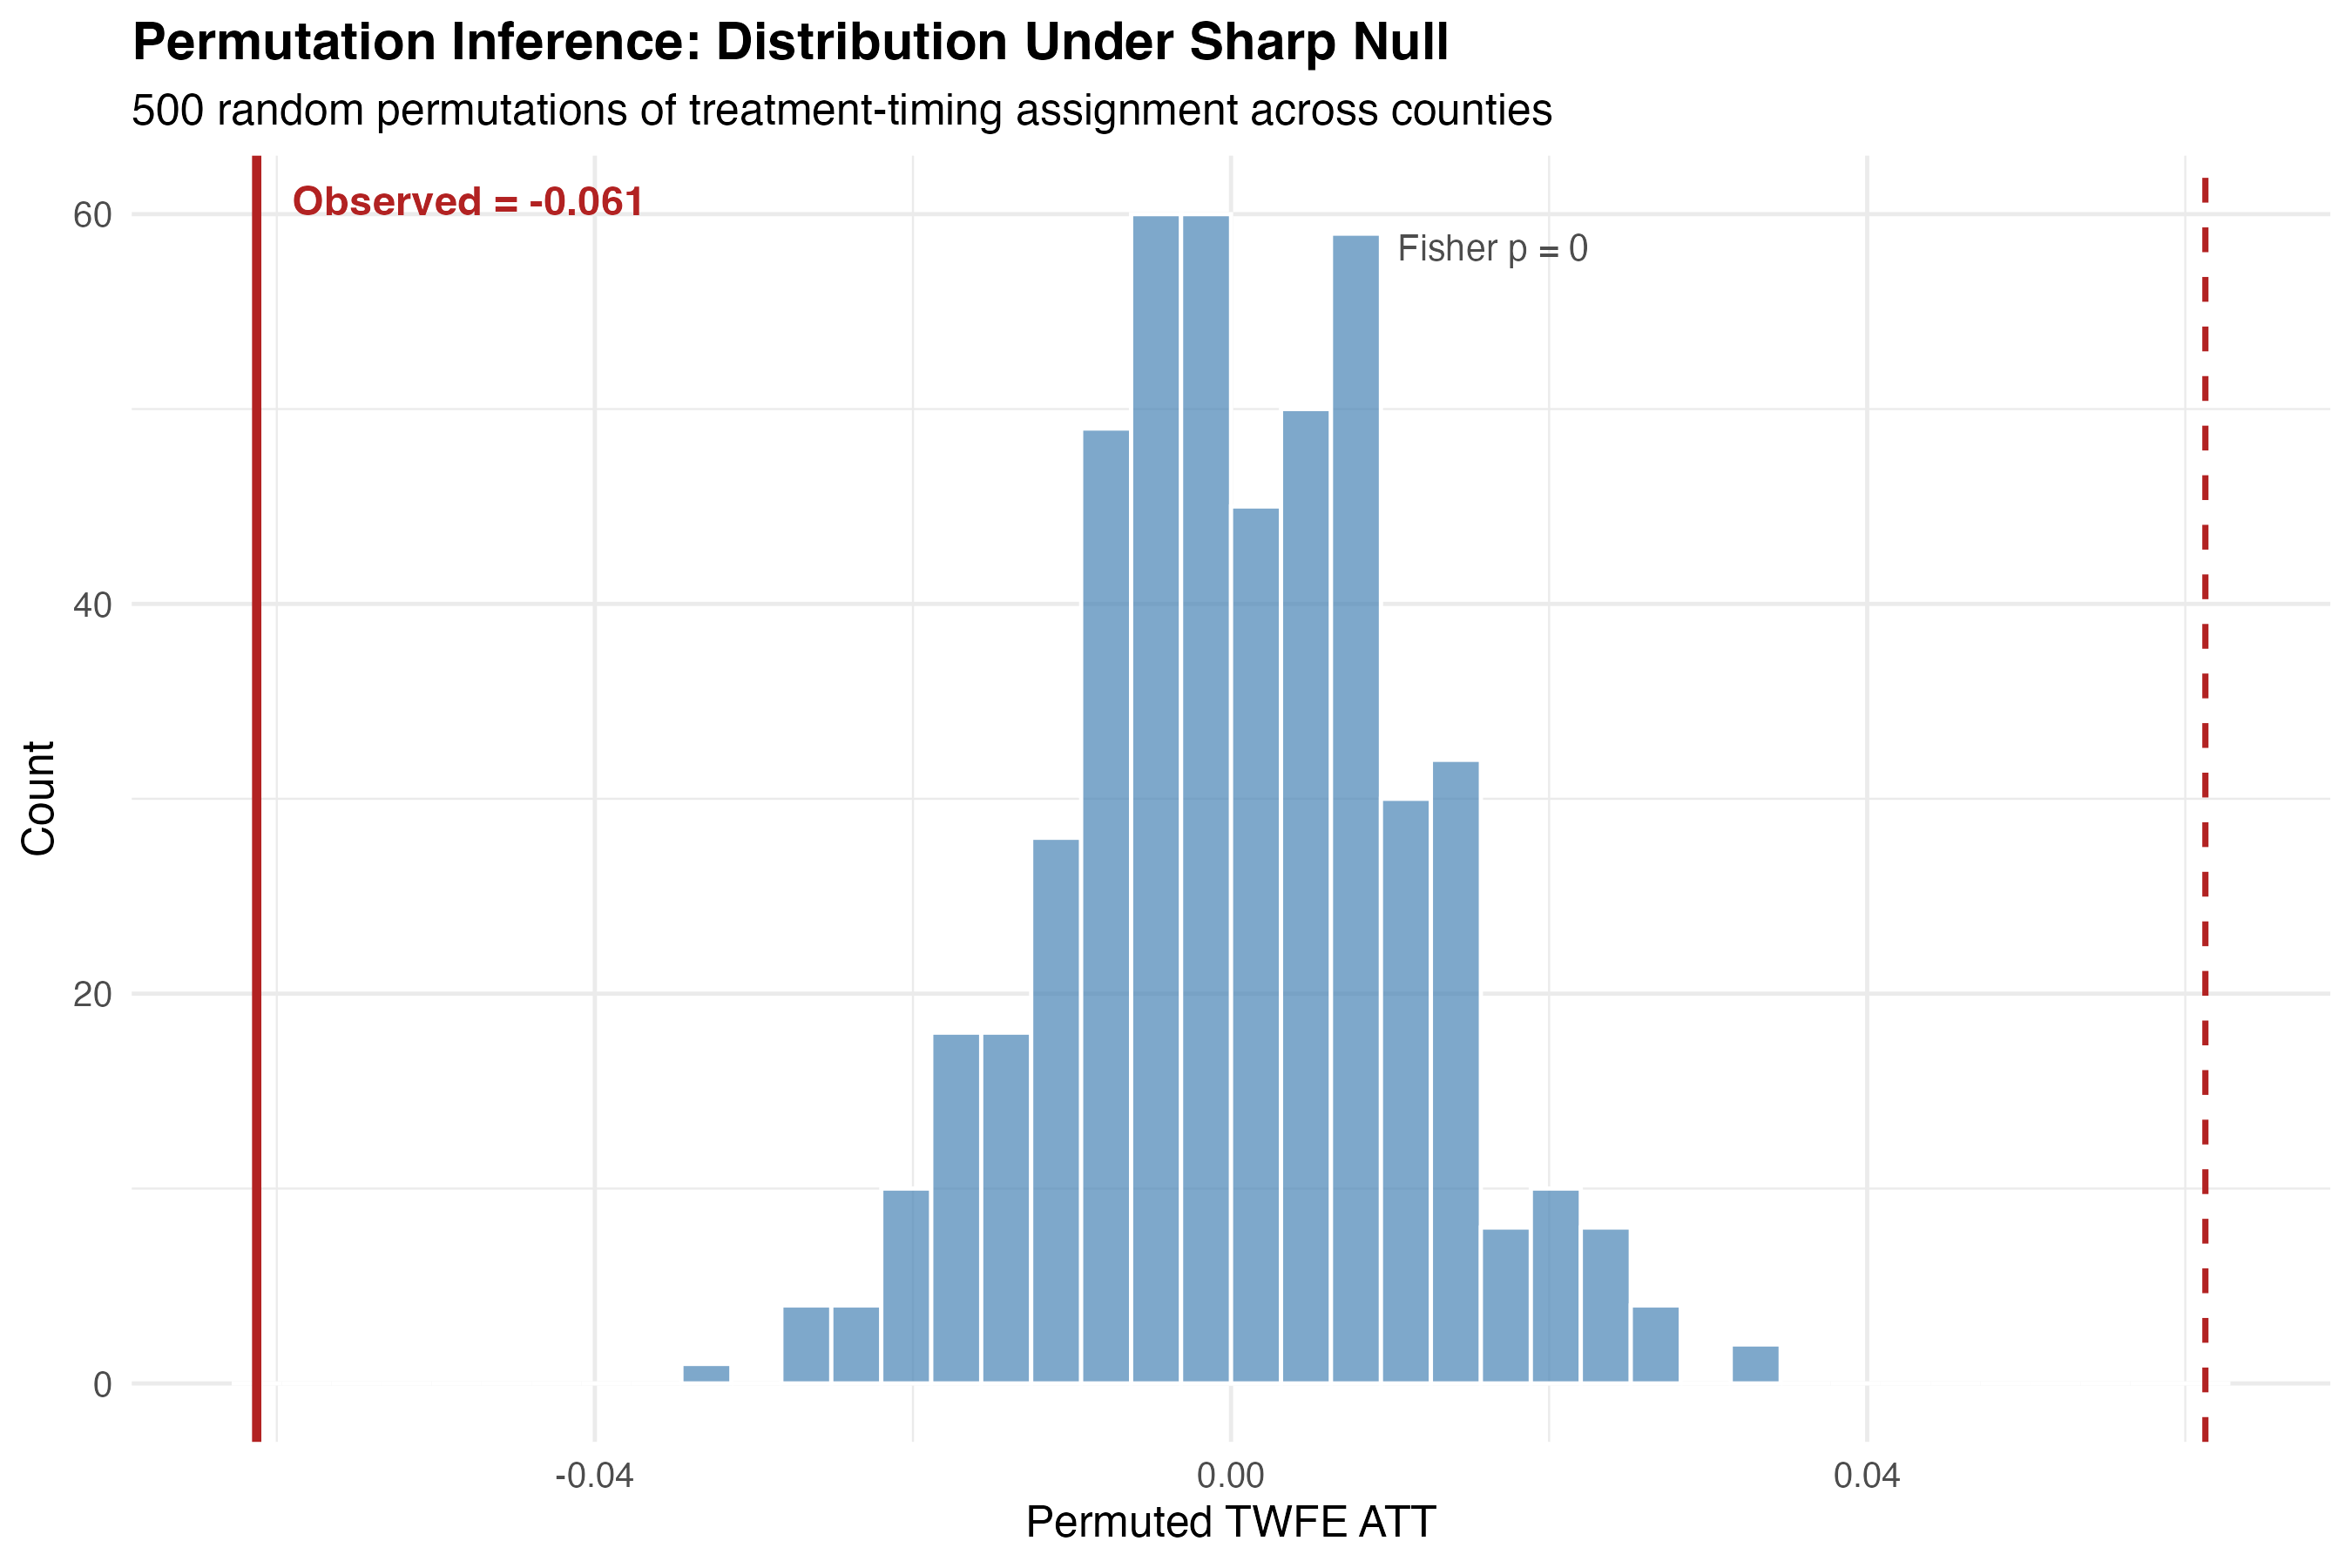
\includegraphics[width=0.65\textwidth]{../outputs/figures/permutation_distribution}

  \vspace{0.3em}
  {\small 500 Fisher randomization draws.  Observed ATT ($-0.061$) far in left tail; $p < 0.002$.}
\end{frame}

\begin{frame}{Heterogeneity Forest Plot}
  \centering
  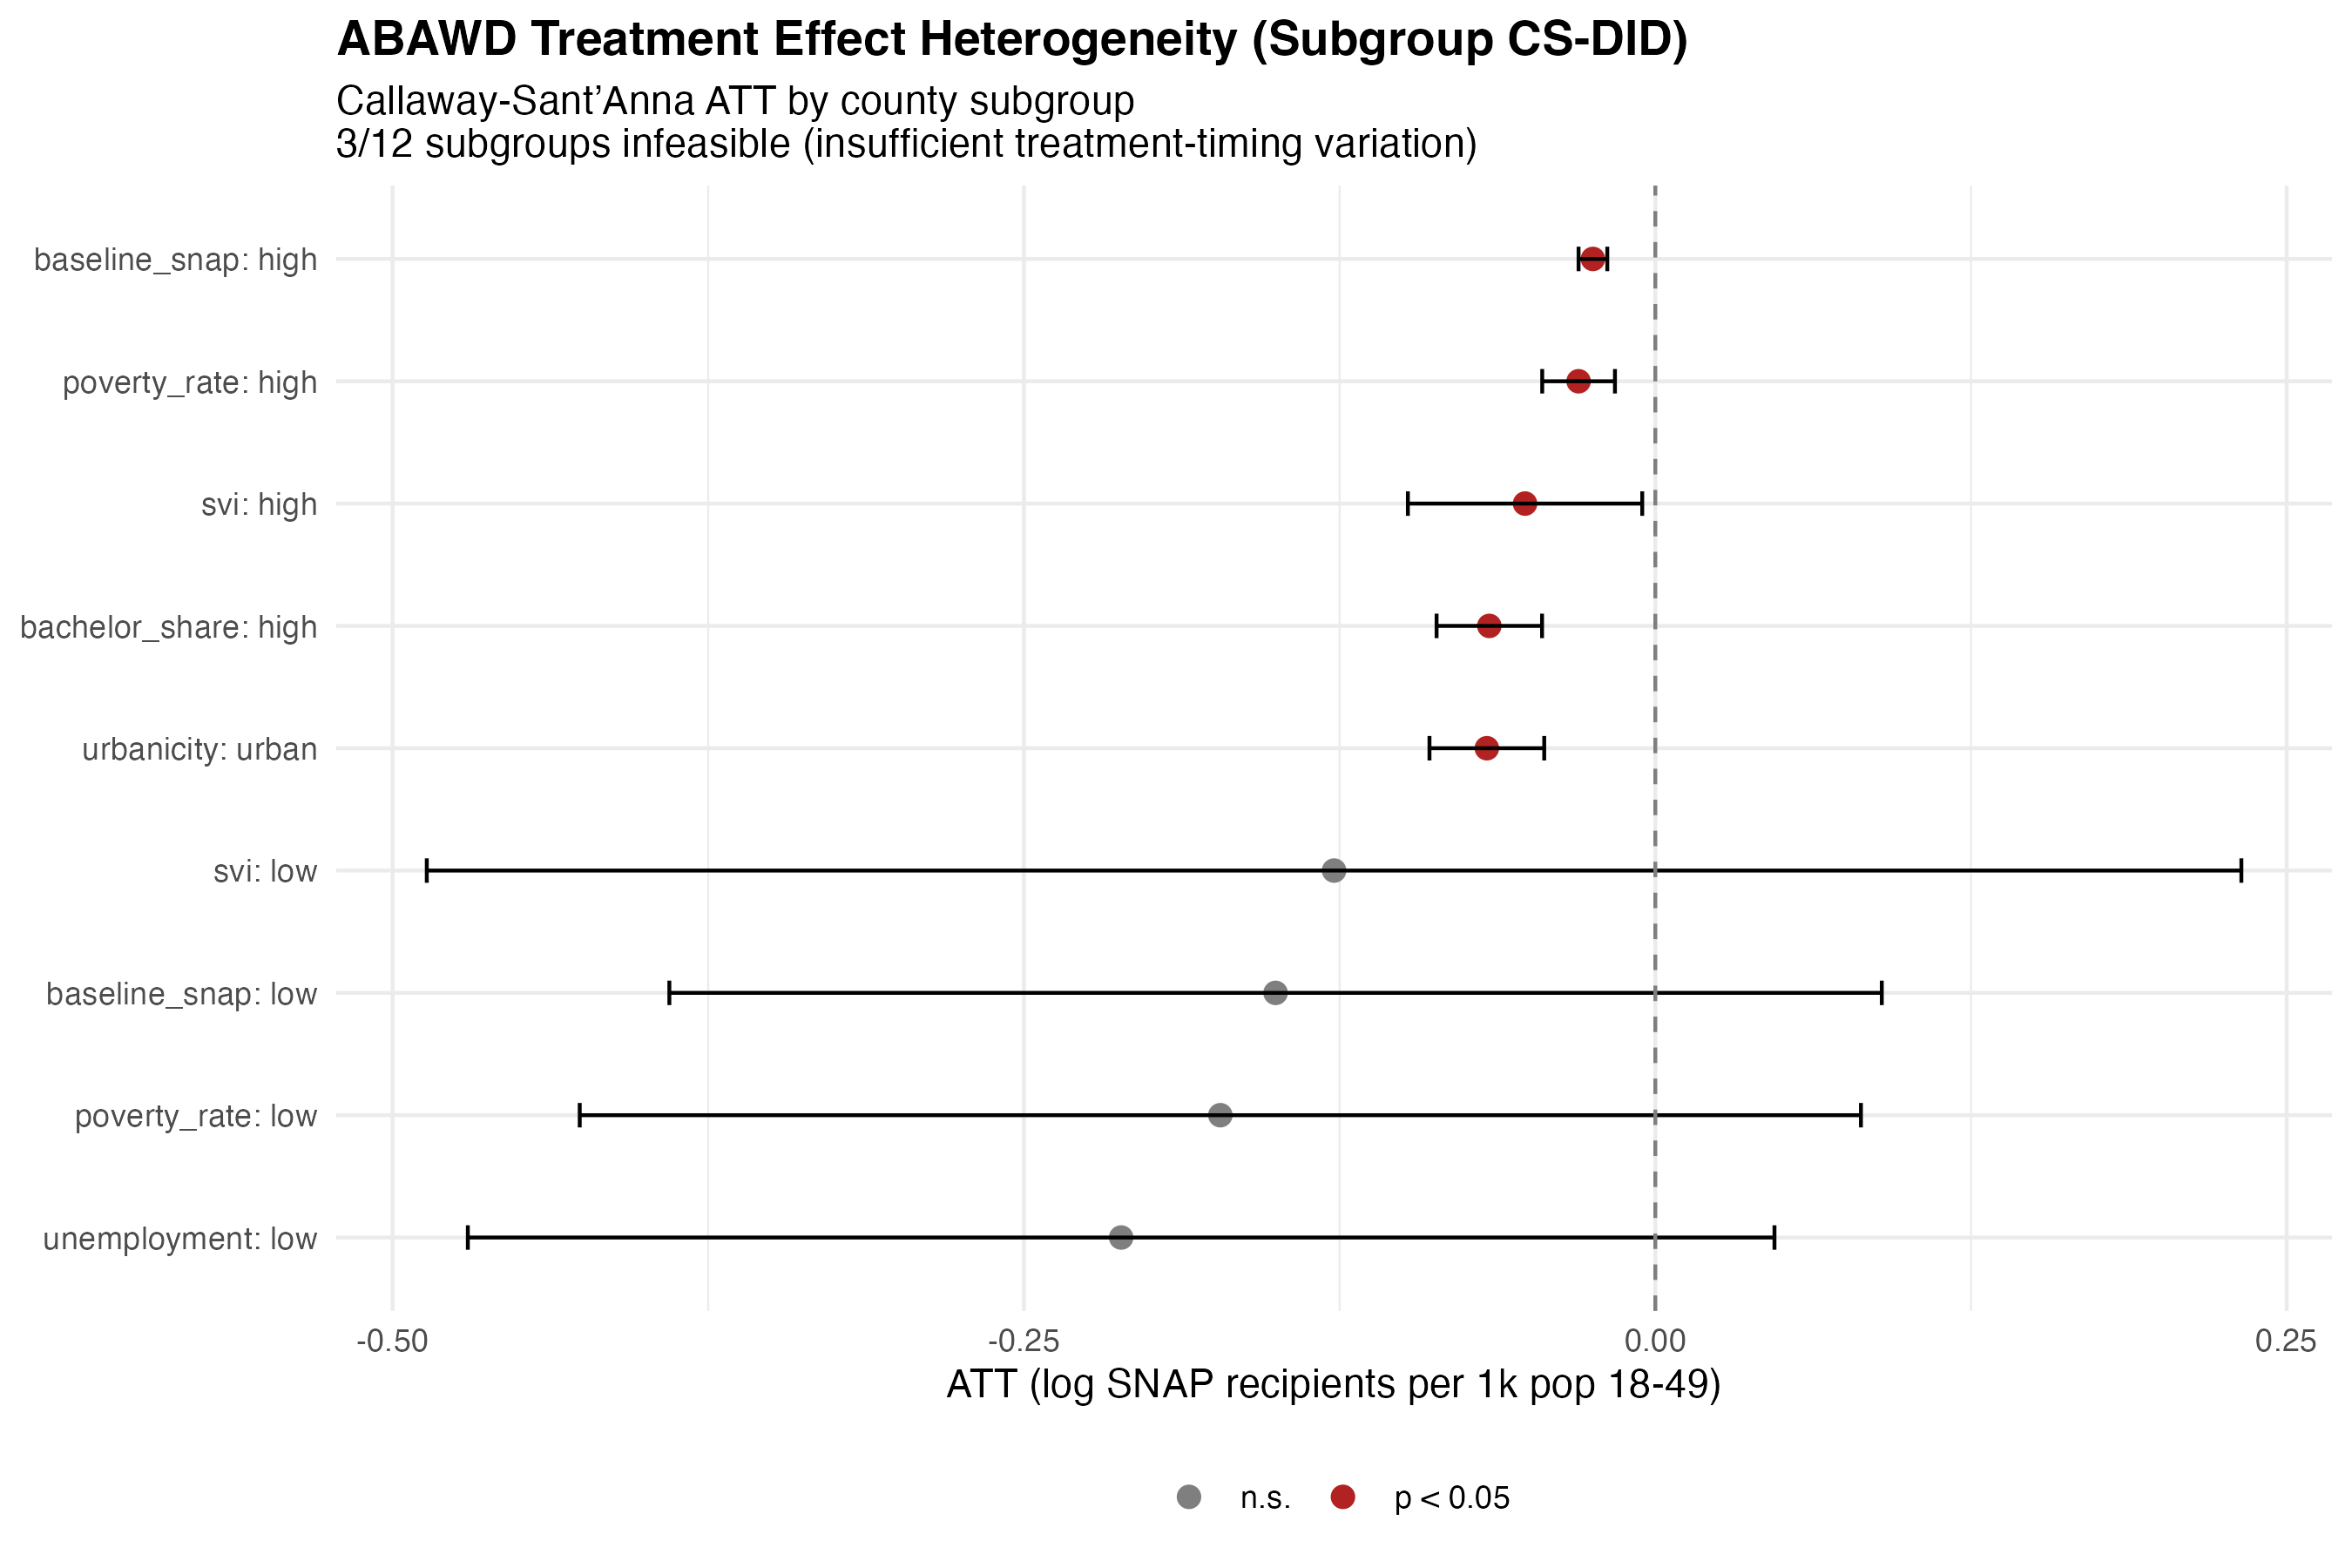
\includegraphics[width=0.75\textwidth]{../outputs/figures/abawd_heterogeneity_forest}
\end{frame}

\end{document}
